\documentclass[11pt,letterpaper]{article}
\usepackage[T1]{fontenc}
\usepackage[utf8]{inputenc}
\usepackage{lmodern}
\usepackage[margin=1in]{geometry}
\usepackage{amsmath,amssymb,amsthm,mathtools}
\usepackage{graphicx,booktabs,array,multirow}
\usepackage{enumitem}
\usepackage[numbers,sort&compress]{natbib}
\usepackage{xcolor}
\usepackage{caption}
\usepackage{placeins}
\usepackage{fancyhdr}
\usepackage{hyperref}
\hypersetup{colorlinks=true,linkcolor=black,citecolor=black,urlcolor=blue!50!black,
  pdftitle={Learning to Match Output Distributions with Batch-Level Rewards},
  pdfauthor={Yash Solanki},pdfsubject={Completed numeric, preference, MMD and energy-distance experiments}}
\urlstyle{same}
\captionsetup{font=small,labelfont=bf}
\setlength{\parskip}{3pt}
\setlength{\parindent}{1.2em}
\setlength{\emergencystretch}{2em}
\setlist{nosep,leftmargin=*}
\pagestyle{fancy}
\fancyhf{}
\fancyhead[L]{\small Learning to Match Output Distributions}
\fancyhead[R]{\small Solanki}
\fancyfoot[C]{\thepage}
\setlength{\headheight}{14pt}
\newcommand{\E}{\mathbb{E}}
\newcommand{\R}{\mathbb{R}}
\newcommand{\KL}{D_{\mathrm{KL}}}
\newcommand{\sg}{\operatorname{stopgrad}}
\newcommand{\ind}{\mathbf{1}}
\newcommand{\nW}{\widetilde W_1}
\newtheorem{proposition}{Proposition}
\title{\vspace{-1.1em}\textbf{Learning to Match Output Distributions\\with Batch-Level Rewards}\\[0.4em]
  \large Numerical Results, Human Preferences, and Conditional Semantic MMD}
\author{Yash Solanki\\University of Washington}
\date{November 22, 2026}

\begin{document}
\maketitle
\begin{abstract}
Stochastic decoding does not ensure that a language model's outputs follow
a requested target distribution. We study batch-level distribution rewards
with leave-one-out REINFORCE and a separate reference-policy KL penalty.
For Qwen2.5-3B numerical sampling, 64,000 supervised examples followed by
250 RL updates and 128,000 generated training responses reduce mean test
histogram KL from 0.227713 to 0.222606 (2.24\%). Evaluation uses 100
held-out prompts with 1,000 draws each; median KL, KS and normalized
Wasserstein improve by 11.29\%, 8.90\% and 9.76\%, with validity near
98.6\% and heterogeneous unseen-family transfer. We then report completed
instruction-model text experiments. Shakespeare unigram/bigram trials
improve empirical matching and their shared training judge, while
HelpSteer2 preference/word-target trials do not establish joint quality
and distribution gains. A stronger scorer-selection audit favors a frozen
8B reward model over the locally fitted 3B Bradley--Terry scorer.
Prompt-conditional semantic MMD uses two acceptable reference answers per
question and fixed full-answer embeddings. The first Gaussian run lowers
held-out discrepancy from 0.39224 to 0.38330 while quality falls slightly.
A calibrated energy-distance run improves matching at 53 updates, but
most of that gain disappears by 200 cumulative updates as quality rises.
All paired 19-question semantic/quality mean-change intervals include zero.
A quality-free four-question fitting diagnostic lowers seen energy
distance 3.8\% and raises unseen distance 1.5\%; post hoc word and character
audits show mixed changes. These single-seed studies provide modest,
protocol-dependent evidence, without exact sampling, reliable joint
semantic/quality gains, or superiority to equal-compute supervised
controls. We give objectives, gradient derivations, achieved budgets,
uncertainty and source records. Larger teacher-reference sets and
conditional-JSD training remain proposed comparisons.
\end{abstract}
\vspace{0.3em}
\noindent\textbf{Code and recorded results:}
\href{https://github.com/YashSolanki2007/llm-random-number-generator}{github.com/YashSolanki2007/llm-random-number-generator}

\section{Introduction}
When asked to sample from a normal distribution, a language model can produce
a plausible number while allocating the wrong probabilities to possible
answers. The relevant property is therefore distributional fidelity across
repeated requests, rather than the plausibility of an individual response.
Temperature-based sampling introduces randomness into token selection, but
does not by itself calibrate the induced distribution over parsed numbers.

This distinction motivates a direct training question: can a model improve its
numerical sampling policy when rewarded for matching the distribution of its
own generated outputs to a specified mathematical target? We study a small,
auditable instance of this question with Qwen2.5-3B and one NVIDIA H200.
The experiment has two completed stages: sampled-target SFT followed by
batch-KL-reward reinforcement learning. A third, direct soft-target KL trainer
has been implemented and tested for pipeline correctness, but has not been
run as a full-model experiment. We report no empirical comparison for that
third method.

The manuscript also documents natural-language extensions using an
instruction-tuned checkpoint: Shakespeare corpus matching, HelpSteer2
human preferences (Section~\ref{sec:helpsteer}), and prompt-conditional
semantic MMD (Section~\ref{sec:mmd}). Section~\ref{sec:newresults}
reports their completed trials, calibrated Gaussian/energy comparisons,
energy continuation, and distribution-only diagnostic. These are separate
protocols, not interchangeable benchmarks. The larger frozen-teacher
reference proposal and conditional-JSD training remain unrun.

Our main empirical finding is incremental: RL lowers average test histogram KL
by 2.24\% relative to SFT. Larger improvements in the median coexist with weak
or negative changes on some distribution families and prompt categories. This
is evidence about one training run, not a demonstration of a general internal
random number generator. The initial hypothesis that preference fine-tuning
causes sampling collapse is also outside the experiment's scope: we start
from a base checkpoint and do not compare pre- and post-RLHF models.

\paragraph{Related work.}
Zhao et al.\ \cite{zhao2026dice} audit native numerical sampling in language
models and distinguish generating many numbers within one response from
independent requests. Baldelli et al.\ \cite{baldelli2026calibration} study
calibration fine-tuning with sampled completions and trie-derived soft
next-token targets. The accompanying controlled-stochasticity discussion by
Kuriakose and Baldelli\ \cite{kuriakose2026blog} motivated the present comparison.
Our pilot instead adds a reward computed from the model's own generated
histogram after SFT; it does not claim priority for distribution-matching
fine-tuning. The optimization follows the score-function REINFORCE framework
\cite{williams1992} and the broader use of simple policy-gradient methods in
language-model post-training \cite{ahmadian2024}. The numerical reward is mathematical,
not human preference feedback as in RLHF \cite{ouyang2022}. We adapt the base
Qwen2.5 model \cite{qwen2025} using LoRA \cite{hu2021lora}. The text
extension uses HelpSteer2 ratings and its separate preference annotations
\cite{wang2024helpsteer,wang2024preference}, with a Bradley--Terry-style
pairwise likelihood \cite{bradley1952}.
For conditional distribution comparison, MMD compares kernel mean
embeddings \cite{gretton2012}; Jensen--Shannon divergence supplies a
bounded alternative on categorical laws \cite{lin1991}. These choices
change the discrepancy, but do not establish that a chosen reference
distribution is correct for a prompt.
The later calibrated-kernel experiments adapt kCGM's distribution-matching
policy gradients and implementation ideas \cite{diamant2026kcgm,kcgmcode};
we claim no novelty for those estimators. Energy-distance comparisons
use the distance/kernel connection of Sejdinovic et al.\ \cite{sejdinovic2013}.

\section{Problem formulation and numeric representation}
Let $c$ be a prompt specifying a distribution family and parameters. An
autoregressive language model defines a completion policy
\begin{equation}
 \pi_\theta(y\mid c)=\prod_{t=1}^{T(y)}
 \pi_\theta(y_t\mid c,y_{<t}),
 \label{eq:policy}
\end{equation}
where $T(y)$ ends at EOS or at the 32-token generation limit. For the capped
generation process, unfinished paths at that limit are also possible outcomes.
The parser $f(y)$ returns a finite number if the whole stripped response is
numeric and terminated with EOS, and returns $\bot$ otherwise. Different text
spellings may parse to the same number. The induced numeric law is
\begin{equation}
 q_\theta(x\mid c)=\sum_{y:f(y)=x}\pi_\theta(y\mid c),
 \qquad x\in\mathcal X\cup\{\bot\}.
 \label{eq:induced}
\end{equation}
Here $\mathcal X$ is the countable set of representable parsed numeric outputs.
EOS and truncation are part of the sampling policy, rather than ignored
formatting details.

Continuous target draws are rounded to five decimal places, with grid spacing
$\delta=10^{-5}$. For an underlying CDF $F_c$, the rounded target mass at a
grid point $z$ is, up to zero-probability rounding ties,
\begin{equation}
 p_\delta(z\mid c)=F_c(z+\delta/2)-F_c(z-\delta/2).
 \label{eq:rounded}
\end{equation}
Discrete targets use their integer-valued probability masses. Canonical
continuous training answers have exactly five decimals, discrete answers are
integers, and negative zero is canonicalized. Evaluation accepts other numeric
spellings; canonical formatting is measured separately.

Numeric validity and support validity are different. A finite numeric response
with EOS is counted as numerically valid even if it lies outside the target
support, or is noninteger for an integer-valued law. Such responses remain in
KS and Wasserstein calculations and are separately flagged. The RL reward
assigns them to its invalid category. For continuous support boundaries, a
half-grid tolerance accounts for target rounding.

At inference, unconstrained token sampling with logits $z_v$ and temperature
$\tau$ uses $\pi_{\theta,\tau}(v)=\exp(z_v/\tau)/\sum_w\exp(z_w/\tau)$.
Our experiments use $\tau=1$ without top-$p$ or top-$k$ truncation. Fine-tuning
changes these probabilities; decoder pseudorandomness selects outcomes.
For comparison, an ordinary numerical sampler can transform
$U\sim\operatorname{Uniform}(0,1)$ into $X=F_c^{-1}(U)$. The present goal is
to improve the language model's induced law, rather than replace that
established sampling construction.

\section{Training methods}
\subsection{Sampled-target SFT baseline}
For each training prompt $c$, we sample 32 independent answers from its target
law using SciPy and append EOS. SFT minimizes completion-token cross-entropy;
prompt and padding tokens are masked. For a minibatch $\mathcal B$,
\begin{equation}
 \mathcal L_{\mathrm{SFT}}(\theta;\mathcal B)=
 -\frac{\sum_{(c,y)\in\mathcal B}\sum_{t=1}^{T(y)}
   \log\pi_\theta(y_t\mid c,y_{<t})}
 {\sum_{(c,y)\in\mathcal B}T(y)}.
 \label{eq:sft}
\end{equation}
This is sampled-answer supervision, not an empirical-distribution RL reward.
The trainable attention projections use LoRA updates
\begin{equation}
 W=W_0+\frac{\alpha_L}{r}BA,
 \qquad r=16,\quad \alpha_L=32,
 \label{eq:lora}
\end{equation}
with frozen base weights. The SFT adapter has 7,372,800 trainable parameters.
LoRA dropout is 0.05 during SFT, and disabled during RL generation and scoring.

\subsection{Target bins and empirical KL reward}
For each prompt, we construct at most 32 numeric bins with approximately equal
target mass. Continuous boundaries are based on rounded target quantiles;
discrete boundaries lie between integer values. A finite discrete support
with at most 32 points is represented exactly. Duplicate or zero-mass
boundaries are removed. Appendix~\ref{app:bins} specifies the construction.

Let $K$ be the number of numeric bins and $B=K+1$ include the invalid category.
The target vector is $P_c=(p_1,\ldots,p_K,p_\bot)$ with
\begin{equation}
 p_j=\Pr_{X\sim p(\cdot\mid c)}(X\in B_j),\qquad p_\bot=0.
\end{equation}
For $N$ fresh independent completions $Y_{1:N}$, let $n_j$ be the count assigned
to category $j$, including invalid completions in the total $N$. With
$\alpha=0.1$, define
\begin{align}
 \widehat q_j&=\frac{n_j+\alpha}{N+\alpha B},\\
 R_N(c,Y_{1:N})&=-\KL(P_c\Vert\widehat Q)
 =-\sum_{j:p_j>0}p_j\log\frac{p_j}{\widehat q_j}.
 \label{eq:reward}
\end{align}
All logarithms are natural. Smoothing prevents infinite costs for unobserved
bins. Although the invalid category has zero target mass, invalid responses
still reduce numeric-bin mass through the denominator. They are never
discarded before computing the reward.

This reward is a finite, smoothed histogram approximation. It is not the exact
KL between a continuous target density and an empirical measure, nor an
unbiased estimate of population histogram KL. The finite-$N$ objective and
its limiting interpretation are given in Appendix~\ref{app:finite}.

\subsection{Policy gradient and leave-one-out credit assignment}
The target-reward objective is
\begin{equation}
 J_N(\theta)=\E_{c}\E_{Y_{1:N}\sim\pi_\theta(\cdot\mid c)}
 [R_N(c,Y_{1:N})].
 \label{eq:batchobjective}
\end{equation}
The score-function identity gives
\begin{equation}
 \nabla_\theta J_N=
 \E\!\left[\sum_{i=1}^N(R_N-b_i)
             \nabla_\theta\log\pi_\theta(Y_i\mid c)\right],
 \quad b_i=R_{N-1}(c,Y_{-i}).
 \label{eq:groupgradient}
\end{equation}
Conditional on $c$, the baseline depends on the other sampled completions
but not on $Y_i$, so its score contribution has zero expectation. In
$R_{N-1}$, both the removed count and the histogram normalization are
recomputed. This estimator is unbiased for the gradient of
Equation~\eqref{eq:batchobjective} under the ideal independent sampling model;
that does not make its reward an unbiased population-KL estimator.

We use scaled advantages $A_i=N(R_N-R_{N-1})$ to compensate for averaging the
sequence losses. The reward is shared by a group, so assigning the same
reward to every action and then subtracting that group's reward mean would
produce zero advantages. No such within-group normalization is used.
The implementation is on-policy REINFORCE, with no PPO clipping, value
network, or GRPO reward normalization. Each rollout batch receives one
optimizer update and is then discarded.

\subsection{Separate reference-policy regularization}
To limit drift, we keep a frozen copy $\pi_{\mathrm{ref}}$ of the initial SFT
adapter, sharing the frozen base model. This reference is not the numeric
target. The full objective is
\begin{equation}
 J_{\mathrm{total}}(\theta)=J_N(\theta)
 -\beta\E_c\KL\!\left(\pi_\theta(\cdot\mid c)
                  \Vert\pi_{\mathrm{ref}}(\cdot\mid c)\right),
 \qquad \beta=0.02.
 \label{eq:fullobjective}
\end{equation}
Define $\ell_i=\log\pi_\theta(Y_i\mid c)-\log\pi_{\mathrm{ref}}(Y_i\mid c)$.
For $G$ prompt groups in an update, the implemented score-function surrogate is
\begin{equation}
 \widehat{\mathcal L}=
 -\frac{1}{GN}\sum_{g=1}^{G}\sum_{i=1}^{N}
 \sg\!\left[N(R_{g,N}-R_{g,-i})-\beta\ell_{g,i}\right]
 \log\pi_\theta(Y_{g,i}\mid c_g).
 \label{eq:surrogate}
\end{equation}
Completion log probabilities include EOS and exclude prompt tokens and
padding. A capped unfinished completion includes every generated token and
receives the invalid reward category. Appendix~\ref{app:reference} derives the
reference-KL gradient. A sampled mean log-ratio can be negative even though
its population expectation is a nonnegative KL.

\subsection{One update in the implemented algorithm}
\noindent\fbox{\begin{minipage}{0.955\linewidth}
\small
\textbf{Batch-KL REINFORCE update}\par\vspace{3pt}
\begin{enumerate}
\item Select $G=2$ prompts, cycling distribution families and sampling a
training configuration within each selected family.
\item For each prompt, generate $N=256$ independent capped completions with
temperature 1, top-$p=1$, and top-$k$ disabled.
\item Parse answers, assign numeric or invalid bins, and compute $R_N$ and
the leave-one-out advantages $A_i$.
\item With dropout disabled, recompute actor and frozen-reference completion
log probabilities and differentiate Equation~\eqref{eq:surrogate} in
microbatches of 16.
\item Clip gradient norm at 1, take one AdamW update, and advance the learning
rate schedule. Save all sampled actions, rewards, and advantages.
\end{enumerate}
\end{minipage}}

\section{Experimental protocol}
\subsection{Model, data, and held-out conditions}
We use the \texttt{Qwen/Qwen2.5-3B} base checkpoint, pinned to revision
\texttt{3aab1f1954e9} (the full identifier is recorded in the configs).
All completed runs use BF16 on a single NVIDIA H200 without base-weight
quantization. Training families are normal, uniform, exponential, beta,
gamma, and binomial. There are 2,000 training configurations and 160
validation configurations, with disjoint exact family/parameter tuples.
The SFT dataset contains 64,000 answers; its validation set has eight answers
per configuration. RL reuses training configurations but samples new model
responses, rather than consuming the target-answer labels.

The test set has 100 prompts: 34 with parameters outside training ranges,
33 from held-out Weibull or Poisson families, and 33 using held-out prompt
wording with familiar families. These conditions are mutually exclusive
categories in this benchmark. Held-out families are absent from training and
validation. The new-wording condition uses one unseen template, not a broad
paraphrase benchmark. All exact family/parameter combinations are disjoint
across splits. Appendix~\ref{app:distributions} lists the laws, parameter
ranges, and prompt templates.

\begin{table}[t]
\centering\small
\caption{Completed training settings. SFT and RL are sequential stages with
different budgets, not equal-compute alternatives.}
\label{tab:settings}
\begin{tabular}{@{}p{0.39\linewidth}p{0.25\linewidth}p{0.25\linewidth}@{}}
\toprule
Setting & SFT & Batch-KL RL\\
\midrule
Updates & 2,000 & 250\\
Training responses & 64,000 target answers & 128,000 model actions\\
Learning rate & $2\times10^{-4}$ & $10^{-5}$\\
AdamW weight decay & 0.01 & 0.01\\
Schedule / warmup & Cosine / 3\% & Cosine / 3\%\\
Update batch & 32 examples & 2 prompts $\times$ 256 draws\\
Rollout batch / gradient microbatch & --- / 32 & 128 / 16\\
LoRA rank / alpha & 16 / 32 & Existing 16 / 32 adapter\\
Attention targets & $q,k,v,o$ projections & Same projections\\
Adapter dropout & 0.05 & Disabled\\
Training seed & 42 & 42\\
Maximum sequence / new tokens & 128 / --- & 128 / 32\\
\bottomrule
\end{tabular}
\end{table}

\subsection{Validation and checkpoint choice}
RL uses the first 12 configurations in the disjoint validation split, with
256 samples each at update 0 and every 25 updates. Their sampling seed
(1731) is fixed and its RNG state isolated from training. The lowest
validation mean KL occurs at update 225. The reported test evaluation uses
the \emph{final} update-250 adapter, not that best validation checkpoint.
The 20-update timing benchmark is discarded; production RL starts afresh
from the original SFT adapter.

\subsection{Independent-request evaluation}
Each model is evaluated on the same 100 prompts with 1,000 generations per
prompt: 100,000 responses per model, 300,000 across base, SFT, and RL. Each
response starts from a fresh context containing only the prompt. Requests
are batched in groups of up to 128 for throughput, with seed 12345,
temperature 1, top-$p=1$, top-$k=0$ (disabled), one beam, repetition penalty
1, and at most 32 new tokens. The models use the same base revision and
evaluation cases. No grammar constraint, rejection sampling, resampling, or
post-hoc correction repairs a response. Fixed seeds and matching settings
do not imply identical response-by-response randomness after policies diverge,
or bitwise reproducibility across hardware.

\subsection{Evaluation metrics}
Numeric validity is the fraction of all requests with a finite numeric-only
answer terminated by EOS. Support violation rates are reported among those
answers. For $m$ valid numeric outputs, let $\widehat F_m$ be their empirical
CDF and $F_\delta$ the discrete or rounded target CDF. We report
\begin{equation}
 D_{\mathrm{KS}}=\sup_x|\widehat F_m(x)-F_\delta(x)|.
 \label{eq:ks}
\end{equation}
The implementation checks both left and right CDF limits at sample values,
which accommodates discrete atoms and repeated outputs. We do not attach
continuous-null KS $p$-values to these discrete/rounded comparisons.

For sorted samples $x_{(1)},\ldots,x_{(m)}$, let $u_i=(i-1/2)/m$.
Wasserstein-1 distance is approximated by midpoint quantile matching and
normalized by the target's 90\% interquantile width:
\begin{equation}
 \widehat W_1=\frac1m\sum_{i=1}^m
 |x_{(i)}-Q_\delta(u_i)|,
 \qquad
 \nW=\frac{\widehat W_1}{Q_c(0.95)-Q_c(0.05)}.
 \label{eq:wasserstein}
\end{equation}
$Q_\delta(u)$ is the rounded underlying quantile for continuous laws and the
discrete quantile for integer laws. This is a numerical approximation, not
the exact continuous Wasserstein integral. Both KS and Wasserstein are
conditional on numeric validity and retain out-of-support numeric values.

Test histogram KL uses Equation~\eqref{eq:reward}, recomputed post hoc from
all 1,000 draws per prompt with the same target bins and pseudocount.
Malformed, unfinished, noninteger discrete, and out-of-support answers remain
in its invalid category. Its sample size differs from the 256-draw training
and validation groups; their absolute KL values should not be compared
directly. Means and medians aggregate prompts with equal prompt weight.

\section{Results}
\subsection{SFT establishes a strong formatting baseline}
Table~\ref{tab:sft} summarizes the initial completed SFT experiment. Numeric
validity rises from 6.838\% to 98.677\%, while conditional distribution
distances decrease substantially. However, the base model reaches the token
limit in 88.625\% of requests, and four base prompts produce no valid
numeric answers. The base distance medians therefore use 96 cases, versus
100 for SFT and RL. These differences preclude attributing the entire
base-to-SFT gain to calibration rather than instruction following,
formatting, and altered effective sample size.

\begin{table}[htbp]
\centering\small
\caption{Pretrained-to-SFT comparison. Distances condition on numeric validity.
The numerical-sampler reference is matched to SFT valid sample counts and
aggregates 20 repetitions per prompt; it is not a separate model.}
\label{tab:sft}
\begin{tabular}{@{}lrrr@{}}
\toprule
Metric & Pretrained & SFT & SciPy reference\\
\midrule
Numeric validity & 6.838\% & 98.677\% & ---\\
Median KS & 0.542819 & 0.139199 & 0.024720\\
Median normalized Wasserstein & 1.685830 & 0.112249 & 0.011348\\
Support violations among numeric & 19.874\% & 1.348\% & ---\\
Prompts without valid samples & 4 & 0 & 0\\
\bottomrule
\end{tabular}
\end{table}

\subsection{RL yields a modest incremental test improvement}
Table~\ref{tab:overall} compares SFT with the final RL adapter on the identical
100-prompt test. Mean histogram KL, the direct aggregate counterpart of the
training cost, decreases by 2.24\%. Median histogram KL decreases by
11.29\%. These different reductions should not be conflated: the typical
prompt's gain is larger than the gain in average KL. Median KS decreases
8.90\% and median normalized Wasserstein decreases 9.76\%; their mean
reductions are 2.83\% and 1.81\%, respectively.

\begin{table}[htbp]
\centering\small
\caption{SFT-to-RL test comparison. All metrics are lower-is-better. Relative
reduction is $100(1-\mathrm{RL}/\mathrm{SFT})$. There are 100 paired prompts
and 1,000 draws per prompt per model.}
\label{tab:overall}
\begin{tabular}{@{}llrrr@{}}
\toprule
Metric & Aggregate & SFT & SFT + RL & Reduction\\
\midrule
Histogram KL & Mean & 0.227713 & 0.222606 & 2.24\% \\
Histogram KL & Median & 0.119134 & 0.105688 & 11.29\% \\
KS distance & Mean & 0.187162 & 0.181865 & 2.83\% \\
KS distance & Median & 0.139199 & 0.126811 & 8.90\% \\
Normalized Wasserstein & Mean & 0.202452 & 0.198792 & 1.81\% \\
Normalized Wasserstein & Median & 0.112249 & 0.101290 & 9.76\% \\
\bottomrule

\end{tabular}
\end{table}

Histogram KL improves on 61 prompts and worsens on 39. Wasserstein improves
on 65 and worsens on 35. KS improves on 59, worsens on 39, and is tied on
two. Numeric validity changes from 98,677 to 98,591 valid responses out of
100,000, a decrease of 0.086 percentage points. Support violations among
numeric answers fall from 1,330 to 1,208 (1.348\% to 1.225\%). Thus the
distributional changes coexist with almost unchanged response validity.

\paragraph{Exploratory uncertainty.}
We resample the 100 paired prompt indices with replacement 10,000 times
(seed 90210), recomputing each aggregate difference. The percentile 95\%
interval for the mean KL difference, RL minus SFT, is
$[-0.008401,-0.001804]$. The median KL interval includes zero, as does the
median Wasserstein interval. The median KS interval is barely negative.
Full intervals appear in Appendix~\ref{app:extended}. These are exploratory
prompt-bootstrap intervals for this fixed experiment, not across-seed
uncertainty or a multiplicity-adjusted confirmation of general benefit.

\subsection{Validation improves non-monotonically}
Mean validation histogram KL changes from 0.070539 at update 0 to 0.065246
at update 250, a 7.50\% decrease. The lowest recorded value is 0.064350 at
update 225. Validation numeric validity is 100\% at all recorded probes.
Figure~\ref{fig:training} shows noisy training groups and a non-monotonic
validation trajectory. The training prompts vary, and validation and test
have different prompt distributions, so these curves do not establish a
smooth or universal calibration improvement. The sequence reference-KL
estimate remains small but noisy; it is a separate quantity from the
histogram target KL.

\begin{figure}[htbp]
\centering
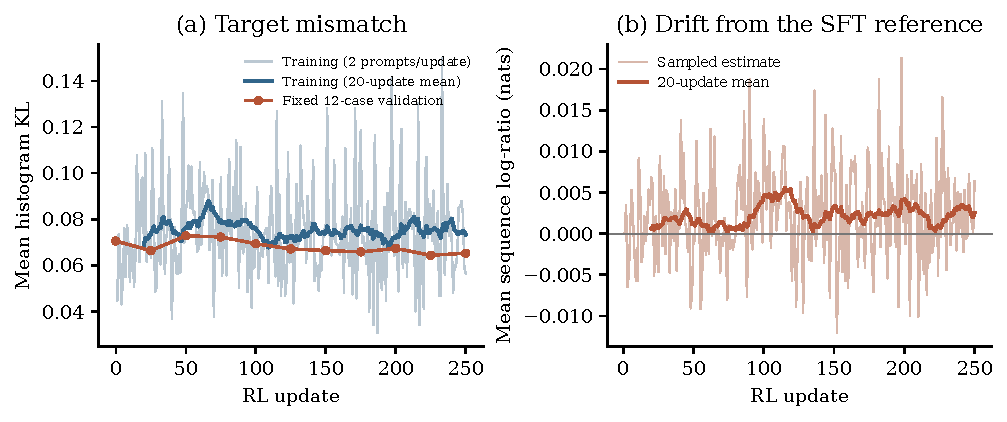
\includegraphics[width=\linewidth]{figures/training.pdf}
\caption{Recorded RL trajectory. Each training point averages two 256-draw
groups; validation uses 12 fixed held-out configurations. The reference
curve estimates $\E\log(\pi_\theta/\pi_{\mathrm{ref}})$ from sampled
completions; negative individual estimates are possible. Lines labeled
20-update mean are trailing moving averages.}
\label{fig:training}
\end{figure}

\subsection{Improvements vary across families and held-out conditions}
Table~\ref{tab:families} shows all eight families. Normal and uniform median
KS decrease by 10.7\% and 15.2\%; exponential and held-out Weibull median
KS increase by 4.5\% and 6.3\%. Held-out Poisson improves 4.0\% on median
KS. Family-level aggregates contain only 10--17 prompts, and combining
them can hide different directions of change.

\begin{table}[htbp]
\centering\small
\caption{Per-family test medians. Stars denote families absent from training
and validation. $n$ is the number of prompts, not the number of draws.}
\label{tab:families}
\begin{tabular}{@{}lr rrrr@{}}
\toprule
& & \multicolumn{2}{c}{KS} & \multicolumn{2}{c}{Normalized Wasserstein}\\
\cmidrule(lr){3-4}\cmidrule(l){5-6}
Family & $n$ & SFT & RL & SFT & RL\\
\midrule
Normal & 12 & 0.0763 & 0.0681 & 0.0559 & 0.0547 \\
Uniform & 12 & 0.1095 & 0.0929 & 0.0610 & 0.0533 \\
Exponential & 12 & 0.1316 & 0.1374 & 0.1883 & 0.1897 \\
Beta & 11 & 0.1112 & 0.1080 & 0.1104 & 0.1005 \\
Gamma & 10 & 0.2170 & 0.2012 & 0.1571 & 0.1361 \\
Binomial & 10 & 0.2724 & 0.2674 & 0.1783 & 0.1693 \\
Weibull$^\star$ & 17 & 0.1387 & 0.1475 & 0.1159 & 0.1128 \\
Poisson$^\star$ & 16 & 0.2282 & 0.2190 & 0.1808 & 0.1785 \\
\bottomrule

\end{tabular}
\end{table}

For unseen parameter ranges, both median KS and Wasserstein improve
(Table~\ref{tab:categories}). The combined unseen-family category worsens
on both medians, even though its mean histogram KL improves slightly.
For new wording, mean histogram KL is nearly unchanged, median
Wasserstein improves slightly, and median KS worsens. Different metrics
therefore support different local conclusions. Numeric validity is 100\%
for unseen-parameter and unseen-family prompts under both policies; for
new wording, it falls from 95.991\% to 95.730\%.

\begin{table}[htbp]
\centering\small\setlength{\tabcolsep}{4pt}
\caption{Held-out category results. KL columns are means; KS and Wasserstein
columns are medians. Test categories are disjoint.}
\label{tab:categories}
\begin{tabular}{@{}lr rrrrrr@{}}
\toprule
& & \multicolumn{2}{c}{Histogram KL} & \multicolumn{2}{c}{KS} &
\multicolumn{2}{c}{Normalized $W_1$}\\
\cmidrule(lr){3-4}\cmidrule(lr){5-6}\cmidrule(l){7-8}
Category & $n$ & SFT & RL & SFT & RL & SFT & RL\\
\midrule
Unseen parameters & 34 & 0.0823 & 0.0717 & 0.1114 & 0.1079 & 0.0826 & 0.0726 \\
Unseen families & 33 & 0.2007 & 0.1961 & 0.1696 & 0.1758 & 0.1410 & 0.1420 \\
New wording & 33 & 0.4045 & 0.4046 & 0.1599 & 0.1690 & 0.1726 & 0.1701 \\
\bottomrule

\end{tabular}
\end{table}

\begin{figure}[!t]
\centering
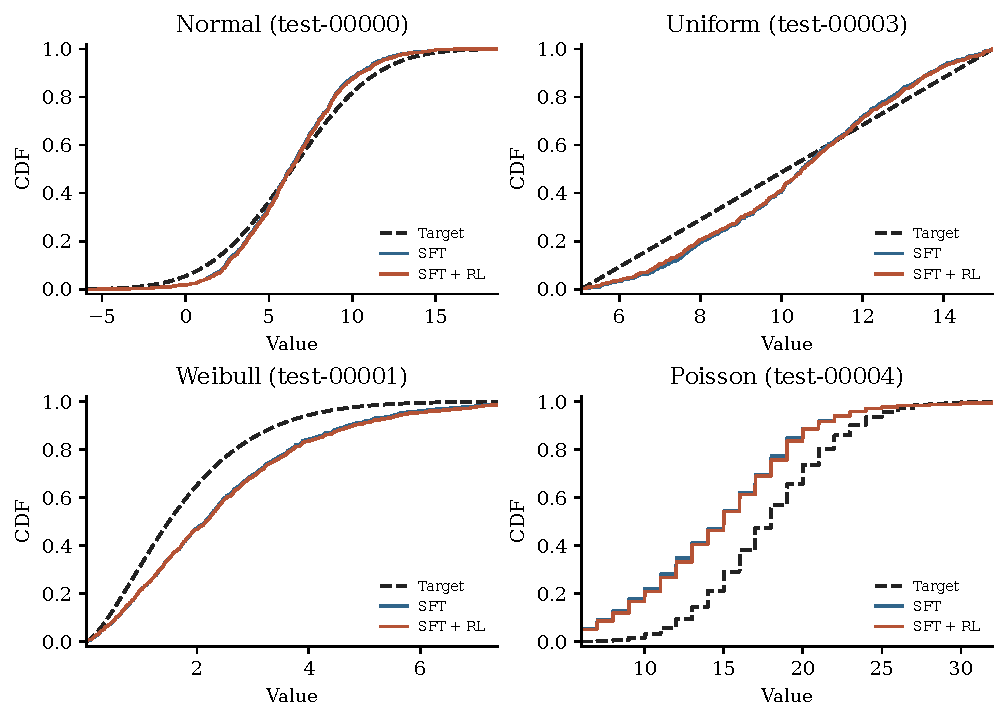
\includegraphics[width=\linewidth]{figures/ecdf.pdf}
\caption{Illustrative empirical CDFs, using the first test case of each of
four displayed families, rather than selecting the largest gains.
Normal and uniform are unseen-parameter cases; Weibull and Poisson are
unseen-family cases. Each curve uses valid numeric responses from 1,000
requests. Horizontal limits span target quantiles 0.001--0.999; complete
metrics retain all numeric outputs. These examples do not summarize all
prompts or certify independence.}
\label{fig:ecdf}
\end{figure}

\subsection{Compute and implementation checks}
The SFT Slurm job takes 4m50s, including a recorded training loop of
253.73 seconds. The RL job takes 22m34s, with 1,329.90 seconds recorded
inside the RL loop and its validation/checkpoint work. Final RL evaluation
takes 5m43s, and the preceding 20-update benchmark takes 2m20s. These
are observed single-H200 durations, excluding scheduler queue time.
They are not throughput guarantees for other workloads.

The local suite passes 44 tests, including numerical KL checks,
enumeration of the toy group-policy gradient, categorical-target
convergence, the reference-KL score gradient, EOS/padding masks, a frozen
reference adapter, and tiny-model checkpoint/resume integration. These
checks support implementation correctness; they are not substitutes for
replicated scientific experiments.

\FloatBarrier
\section{Human-preference extension: HelpSteer2 methods}
\label{sec:helpsteer}
\noindent\textbf{Protocol scope.} This section preserves the initial
HelpSteer2 reward-model and unigram-RL design. The later semantic-MMD
profile in Section~\ref{sec:mmd} uses a different frozen scorer,
reference subset, generation limit, and conditional batching. Its
settings must not be inferred from this earlier design.

\noindent\textbf{Status of evidence.} This section records the original
prepared-data and reward-model design, including the larger configured
policy profile. Section~\ref{sec:newresults} reports the completed subset
trials and subsequent corrected profiles with their actual budgets and
scorer-selection audit. Preparation counts below are not achieved
policy-training counts; later configurations are stated separately.

\subsection{Dataset and prompt-disjoint preparation}
We replace a synthetic mathematical target with natural-language prompts
and human feedback from \texttt{nvidia/HelpSteer2}
\cite{wang2024helpsteer,wang2024preference}. We use both the attribute-rated
responses and the separate \texttt{preference/preference.jsonl.gz} pairs,
pinned to dataset revision \texttt{990b2711a361}. The full revision and
source-file hashes appear in the supplementary protocol record. The
dataset is distributed under CC-BY-4.0; its preference annotations are
human feedback, not synthetic judgments generated for this experiment.

Before splitting, the preparation code collapses whitespace in the prompt
text and hashes the result. Whitespace-equivalent prompts therefore stay
together. One pair is retained per canonical prompt, and an official
validation occurrence takes priority over a duplicate training occurrence.
This grouping does not establish semantic deduplication of differently
worded prompts. Full multi-turn context is parsed from the source
User/Assistant markers and preserved in the Qwen chat template.

The original training partition is divided by a deterministic prompt-hash
rule: hash modulo four equal to zero reserves a prompt for the policy/PMF
pool, and the other residues reserve it for reward-model training.
The nominal allocation is 25\%/75\% before further policy eligibility
filters, not an exact fraction after filtering. The original validation
partition supplies disjoint reward validation, policy validation, and
policy test prompts. Eligible policy evaluation prompts are sorted,
shuffled with seed 42, and assigned to validation and test; the remaining
original validation prompts supply reward validation.

Both candidate responses must have at least 90\% ASCII among alphabetic
characters. This is a language-selection heuristic rather than an English
classifier. Chat-formatted prompts must have at most 384 tokens, and
each complete candidate reward-model input at most 1,024 tokens. Source
answers exceeding a limit are excluded rather than silently truncated.
Policy/reference eligibility additionally requires a non-tied preferred
answer, at most 256 response tokens, with human coherence, correctness,
and helpfulness ratings each at least 3 on the 0--4 scale. Reward-model
training does not require this additional preferred-reference filter.
These choices define a selected short-answer subset, not the complete
HelpSteer2 benchmark.

\begin{table}[htbp]
\centering\small
\caption{Verified prepared HelpSteer2 subset. Splits are disjoint by canonical
prompt hash. These counts do not indicate completed training or evaluation.}
\label{tab:helpsteerdata}
\begin{tabular}{@{}lrp{0.52\linewidth}@{}}
\toprule
Subset & Count & Use\\
\midrule
Reward training & 5,095 pairs & Fit the scalar preference reward model\\
Reward validation & 295 pairs & Select reward checkpoint and normalize scores\\
Policy training & 533 prompts & Sample actions for both policy arms\\
Preferred-response reference & 533 responses & Build the training-only word PMF\\
Policy validation & 16 prompts & Periodic policy diagnostics\\
Policy test & 32 prompts & Final base/quality/KL comparison\\
\bottomrule
\end{tabular}
\end{table}

The reward-training and reward-validation sets include 1,225 and 79 ties,
respectively; reward validation therefore has 216 non-tied pairs.
The reference PMF uses only the 533 preferred policy-training responses.
Reward-training and policy-training prompts are disjoint; evaluation
responses and labels enter neither reward training nor PMF construction.
Held-out human ratings do affect evaluation-subset eligibility, which must
be considered when interpreting eventual results. Human-written preference
rationales are not inputs to the trained reward scorer. Neither the prior
Shakespeare corpus nor a Shakespeare-trained adapter supplies data or
initialization for this extension.

\subsection{Bradley--Terry preference reward model}
Let a human-labeled pair be $(c,y_1,y_2,s)$, where positive source preference
strength $s$ prefers \emph{response two}, negative $s$ prefers response one,
and zero is a tie. A separate
\texttt{Qwen2.5-3B-Instruct} sequence classifier produces a scalar score
$r_\phi(c,y)$. With $\sigma(z)=(1+e^{-z})^{-1}$ and
$\Delta_\phi=r_\phi(c,y_2)-r_\phi(c,y_1)$, the pairwise model is
\begin{equation}
 P_\phi(y_2\succ y_1\mid c)=\sigma(\Delta_\phi),
 \qquad t(s)=\frac{1+\operatorname{sign}(s)}{2}.
 \label{eq:btprob}
\end{equation}
We minimize binary cross-entropy with this soft target:
\begin{align}
 \mathcal L_{\mathrm{BT}}(\phi)
 &=-\E_{\mathcal D_{\mathrm{RM}}}
  [t\log\sigma(\Delta_\phi)+(1-t)\log(1-\sigma(\Delta_\phi))],
 \label{eq:btloss}\\
 \frac{\partial\mathcal L_{\mathrm{pair}}}{\partial\Delta_\phi}
 &=\sigma(\Delta_\phi)-t.
 \label{eq:btgradient}
\end{align}
The sign convention matters: a positive label should increase the second
answer's score relative to the first. Preference-strength magnitude is
not interpreted as a probability or a loss weight. Ties use $t=1/2$,
whose pair loss is minimized at equal scores. This is soft-label treatment
of ties, not a separate three-outcome tie-probability model. The pair
likelihood depends on score differences and is invariant to a shared
additive score shift.

The reward model has attention LoRA rank 16, alpha 32, no dropout, and a
trainable scalar score head. The planned fit is one shuffled epoch over
5,095 pairs, effective batch 32 pairs, microbatch four pairs, AdamW learning
rate $2\times10^{-5}$, cosine decay, approximately 5\% warmup, weight
decay 0.01, and gradient-norm clipping at one. A full epoch would contain
160 updates; the elapsed-time budget can stop it earlier. Model selection
uses reward-validation pair loss. Before policy training, the selected
model must have non-tied validation accuracy greater than 50\%, validation
score standard deviation above $10^{-6}$, and at least one training
update. This is a technical gate, not a significance test or certification
of generated-answer quality. A subsequent stronger selection audit and
its outcomes appear in Section~\ref{sec:newresults}.

For the selected reward model, pool both candidates' raw scores on reward
validation and fix their mean $m_\phi$ and population standard deviation
$s_\phi$. The frozen quality reward for a policy action is
\begin{equation}
 r_Q(c,y)=\ind\{y\text{ terminates with EOS}\}\,
 \sigma\!\left(\frac{r_\phi(c,y)-m_\phi}{\max(s_\phi,10^{-6})}\right).
 \label{eq:qualitytransform}
\end{equation}
The implementation clips the standardized score to $[-30,30]$ before
applying the sigmoid. This bounded utility is not a calibrated human
win probability; centering and scaling do not supply that guarantee.
The scorer sees the complete prompt and answer, without human rationales
at inference. Its parameters and normalization remain fixed during RL.

\subsection{Training-only word target and global histogram}
Let $\mathcal R$ be the 533 preferred policy-training responses. Words
are extracted using ASCII alphabetic runs with optional internal straight
or curly apostrophes, lowercased, and curly apostrophes normalized to
straight ones. No stemming or stopword removal is applied. The vocabulary
$\mathcal V$ consists only of reference words. A single pooled unigram
target is
\begin{equation}
 p_w=\frac{C_{\mathcal R}(w)}{\sum_{v\in\mathcal V}C_{\mathcal R}(v)},
 \quad w\in\mathcal V,\qquad p_{\mathrm{UNK}}=0.
 \label{eq:wordtarget}
\end{equation}
The prepared reference contains 57,251 extracted word occurrences and
7,593 distinct word types. These are corpus statistics, not policy
measurements. This is a marginal word-frequency target across responses, not a
prompt-conditional law or a measure of semantic correctness.

For a global batch $\mathcal B=(Y_1,\ldots,Y_M)$, collect each passage's
word-count vector $\mathbf c_i$ on $\mathcal V\cup\{\mathrm{UNK}\}$.
Unseen words enter UNK. An empty extracted passage contributes one UNK
count; unfinished passages retain all their observed words. Let
$V=|\mathcal V|$, $C_w=\sum_i c_{i,w}$, and $L=\sum_w C_w$. The
total smoothing mass is fixed at $a=1$, unlike the numerical experiment's
per-category pseudocount 0.1:
\begin{equation}
 \widehat q_w=\frac{C_w+a/(V+1)}{L+a},\qquad
 D_{\mathrm{word}}(\mathcal B)=
 \sum_{w:p_w>0}p_w\log\frac{p_w}{\widehat q_w}.
 \label{eq:wordkl}
\end{equation}
The denominator includes UNK counts. Because counts pool words, long
passages contribute more mass, and even a perfectly matched population
PMF has sample-count-dependent estimated KL. Future comparisons must
report lengths and use count-matched post-hoc diagnostics; a lower finite
KL alone is not sufficient evidence of better lexical calibration.

\subsection{Controlled policy arms and the combined objective}
The two independent actor adapters start from the same pinned
\texttt{Qwen2.5-3B-Instruct} checkpoint and seed 42. One arm uses quality
reward only, $\lambda=0$; the other adds word-distribution control,
$\lambda=0.1$. Both use the same frozen learned reward and training
prompts. The unadapted instruction checkpoint, evaluated with actor
adapters disabled, is the third comparison condition. Unlike numerical
RL, this stage does not initialize from the numerical SFT adapter.

Writing $\pi_0$ for the unadapted instruction policy, the objective is
\begin{align}
 J_\lambda(\theta)=
 &\E_{\mathbf c,Y_{1:M}}
 \left[\frac1M\sum_{i=1}^{M}r_Q(c_i,Y_i)
                    -\lambda D_{\mathrm{word}}(Y_{1:M})\right]\nonumber\\
 &-\beta\E_c\KL\!\left(\pi_\theta(\cdot\mid c)
                         \Vert\pi_0(\cdot\mid c)\right),
 \qquad \beta=0.002.
 \label{eq:helpsteerobjective}
\end{align}
Here $\mathbf c$ is the batch of prompts. The Bradley--Terry likelihood
fits the reward model offline; on-policy REINFORCE updates the actor
later. These are different training stages. The numeric target KL,
word-target KL, and reference-policy KL also remain distinct quantities.

For $D=D_{\mathrm{word}}(\mathcal B)$ and
$D_{-i}=D_{\mathrm{word}}(\mathcal B\setminus\{Y_i\})$, the global
leave-one-passage-out credits are
\begin{align}
 A_i^Q&=r_Q(c_i,Y_i)-\frac{1}{M-1}\sum_{j\ne i}r_Q(c_j,Y_j),\\
 A_i^D&=M(D_{-i}-D),\\
 \widehat{\mathcal L}_{\mathrm{actor}}&=
 -\frac1M\sum_i\sg\!\left[A_i^Q+\lambda A_i^D
       -\beta\log\frac{\pi_\theta(Y_i\mid c_i)}{\pi_0(Y_i\mid c_i)}\right]
       \log\pi_\theta(Y_i\mid c_i).
 \label{eq:helpsteersurrogate}
\end{align}
Removing a passage removes its entire count vector and changes the
histogram's word-count denominator. Advantages are computed on the
global batch gathered from both GPU ranks, not on separate per-rank
histograms. Equal local batches and DDP averaging yield the global mean
gradient. Quality and weighted distribution-advantage RMS values are
logged separately; no within-batch variance normalization rescales them.

\begin{table}[htbp]
\centering\small
\caption{Original larger HelpSteer2 configuration, not the achieved subset
trial. Completed-run counts and overrides appear in Section~\ref{sec:newresults}.}
\label{tab:helpsteersettings}
\begin{tabular}{@{}lp{0.62\linewidth}@{}}
\toprule
Setting & Configuration\\
\midrule
Actor budget & Up to 600 updates, 16 global passages/update (9,600 if complete)\\
Prompt grouping & Two prompts/update, eight completions per prompt across two GPUs\\
Actor adaptation & Attention LoRA rank 16, alpha 32, dropout disabled\\
Actor optimizer & AdamW, learning rate $5\times10^{-6}$, weight decay 0.01\\
Schedule & Cosine decay, 40 warmup updates, gradient clipping at one\\
Gradient microbatch & Two passages per GPU microbatch\\
Sampling & Temperature 1, top-$p=1$, top-$k$ disabled, at most 384 new tokens\\
Word-KL weight & $\lambda\in\{0,0.1\}$, not tuned for the new learned reward\\
Policy validation / test & 16 / 32 prompts, two draws per prompt\\
Reference penalty & Reverse sequence KL to instruction base, coefficient 0.002\\
\bottomrule
\end{tabular}
\end{table}

\subsection{Original evaluation design and interpretation}
The configured policy validation uses 32 passages per probe and final
test uses 64 passages per condition. Initial and final policies use
matched per-rank seeds and decoding settings. A separate pinned
Qwen2.5-7B-Instruct auditor rates coherence, readability, and prompt
fulfillment on final test generations. The auditor never supplies the
training reward. It computes expected ratings conditional on tokens
1--5, records their total original probability, and rejects a rating
whose token mass is below 0.01. It is a separate same-family model,
not human evaluation or an independently validated quality standard.

The intended analysis compares the instruction baseline, quality-only
actor, and quality-plus-KL actor on learned reward, external rubric
scores, word KL, UNK rate, EOS termination, and length. Actual training
counts and stop reasons must be included: an elapsed-time cutoff can
leave either arm below 600 updates, weakening an equal-compute
interpretation. The reward fit has a 55-minute elapsed cutoff within a
one-H200 one-hour allocation; each sequential policy job has a
105-minute training cutoff within a two-H200 two-hour allocation,
reserving time for evaluation. These are configured limits, not measured
runtimes. The recorded subset trials and later corrected runs in
Section~\ref{sec:newresults} supersede this profile's pending status;
the full 600-update design is not a completed result.

Training a reward from human labels makes its supervision human-derived;
it does not make generated policy outputs human-validated. A future
positive result would require improvements that survive length/count
controls and do not merely exploit the learned scorer or its word
reference. Multi-seed comparisons and human evaluation would still be
needed. The completed trials do not establish a reliable joint gain.

The source archive's \texttt{supplementary/helpsteer-protocol.json} records
the full dataset and model revisions, prepared-file checksums, split and
tie counts, reference-vocabulary statistics, config, and implementation
hashes. Completed performance records are supplied separately under
\texttt{supplementary/new-results/}.

\FloatBarrier
\section{Prompt-conditional distribution matching with MMD}
\label{sec:mmd}
\noindent\textbf{Evidence status.} This section gives the original
conditional-MMD method and preparation checks. Completed policy results,
calibrated-kernel follow-ups, and diagnostics appear in
Section~\ref{sec:newresults}. This section distinguishes the
implemented two-reference target from the earlier proposal to generate
larger reference sets with an existing frozen teacher. JSD is documented
as a comparison candidate, not an executed conditional training arm.

\subsection{Separating reference choice from discrepancy choice}
A single word PMF pooled across unrelated questions may reward vocabulary
that is inappropriate for an individual answer. Replacing KL with a
bounded or kernel discrepancy does not repair that target mismatch.
The conditional proposal therefore makes two separate choices:
\begin{enumerate}
\item Define a reference distribution for the exact prompt or conversation.
\item Compare generated answers with that reference using a categorical
discrepancy such as JSD, or a feature-space discrepancy such as MMD.
\end{enumerate}
For example, answers to ``What is a Jupyter notebook?'' should be compared
with valid answers to that question, not with pooled vocabulary from
unrelated programming tasks. Features may capture lexical frequencies,
code/prose proportions, formatting, or semantic embeddings. Their choice
defines which properties are controlled; these targets are not
interchangeable notions of successful sampling.

\subsection{Implemented reference subset: two acceptable answers per question}
The current implementation avoids new teacher generation. Starting from
the prepared programming split (228 training, 16 validation, 32 test
prompts), it retains questions with exactly two distinct source answers
whose human coherence, correctness, and helpfulness ratings are each
at least 3 on the 0--4 scale. These answers are model-written and
human-rated, not newly collected human-written demonstrations.
The filtered counts are shown in Table~\ref{tab:mmddata}.

\begin{table}[htbp]
\centering\small
\caption{Verified conditional-MMD preparation statistics. Reference answers
are cached source examples; none is a new student or teacher generation.}
\label{tab:mmddata}
\begin{tabular}{@{}lrr@{}}
\toprule
Split & Exact questions & Reference answers\\
\midrule
Training & 102 & 204\\
Validation & 10 & 20\\
Test & 19 & 38\\
\midrule
Total & 131 & 262\\
\bottomrule
\end{tabular}
\end{table}

Splits inherit the programming dataset's conversation-family separation.
The implementation additionally keys every comparison by its exact
canonical conversation ID, rather than by topic or a shared opening.
Training rejects held-out reference IDs; validation/test references are
used only to evaluate their corresponding questions. The original
programming word PMF remains a training-only diagnostic and is not the
semantic optimization target.

Let $a_{c,1},a_{c,2}$ denote the two acceptable answers and $e(a)$ their
frozen embeddings. The actual target is
\begin{equation}
 P_c^{\mathrm{ref}}=\tfrac12\delta_{e(a_{c,1})}
                        +\tfrac12\delta_{e(a_{c,2})}.
 \label{eq:mmdtarget}
\end{equation}
Equal weights are an experimental choice. Two acceptable answers do not
estimate the frequencies of all valid human answer styles. This target
therefore represents two prototypes, not a recovered human distribution.

\subsection{Frozen full-answer features and the configured kernel}
The encoder is the pinned
\texttt{sentence-transformers/all-MiniLM-L6-v2}, which provides
384-dimensional representations \cite{minilmcard}. Encoder weights stay
frozen. To avoid dropping long-answer tails, tokenization is performed
without truncation, followed by nonoverlapping chunks fitting within
256 encoder tokens including special tokens. Each chunk has
attention-masked mean pooling and unit normalization. Chunk vectors
are combined using their content-token counts as weights, then
renormalized:
\begin{equation}
 u_j=\frac{\operatorname{MeanPool}(h_j)}
              {\|\operatorname{MeanPool}(h_j)\|_2},\qquad
 e(a)=\frac{\sum_j L_j u_j}{\|\sum_j L_j u_j\|_2},
 \label{eq:chunkembedding}
\end{equation}
where $L_j$ is the chunk's content length, with weight one for an empty
chunk. This preserves all visible token chunks, but averaging can lose
global order and dependencies. It is not a proof that code semantics
or correctness are preserved.

The kernel is a mixture of three Gaussian RBF kernels:
\begin{equation}
 k(u,v)=\frac13\sum_{s\in\{0.5,1,2\}}
      \exp\!\left(-\frac{\|u-v\|_2^2}{2b^2s^2}\right).
 \label{eq:mmdkernel}
\end{equation}
The fixed base bandwidth squared is the median nonzero within-question
squared distance between the two training-reference embeddings only:
$b^2=0.2786315084$. No validation/test pair sets this bandwidth.
The median training-pair cosine similarity is 0.8606843. These values
describe the cached reference representation, not model-generation
quality. Both the encoder and reference vectors remain fixed in RL;
new student answers still require encoder inference.

\subsection{Population MMD and the implemented finite estimator}
For independent reference features $X,X'\sim P_c$ and generated
features $Z,Z'\sim Q_{\theta,c}$, the squared MMD is
\begin{align}
 \operatorname{MMD}_k^2(P_c,Q_{\theta,c})
 &=\|\mu_{P_c}-\mu_{Q_{\theta,c}}\|_{\mathcal H_k}^2\nonumber\\
 &=\E k(X,X')+\E k(Z,Z')-2\E k(X,Z),
 \label{eq:mmdpopulation}
\end{align}
where $\mu_P=\E_{X\sim P}k(X,\cdot)$ is the kernel mean embedding
\cite{gretton2012}. The two within-distribution terms and the cross term
compare both spread and cross-group similarity. For suitable
characteristic kernels, zero population MMD identifies equality of
feature distributions. A noninjective text encoder can still map
different or incorrect answers to similar features, so equality in
feature space does not imply equality of text distributions or correctness.

For $n$ generated features $z_1,\ldots,z_n$ and $m=2$ fixed reference
features $x_1,x_2$, the implementation uses
\begin{equation}
 \widehat D_U=
 \frac{\sum_{i\ne j}k(z_i,z_j)}{n(n-1)}
 +\frac{\sum_{a,b=1}^{m}k(x_a,x_b)}{m^2}
 -\frac{2\sum_{i=1}^{n}\sum_{a=1}^{m}k(z_i,x_a)}{nm}.
 \label{eq:mmdestimator}
\end{equation}
Only the generated self-term is a U-statistic; the reference term
includes diagonal terms because it defines the fixed empirical target
in Equation~\eqref{eq:mmdtarget}. Conditional on that target and
independent generated answers, $\E\widehat D_U=
\operatorname{MMD}_k^2(P_c^{\mathrm{ref}},Q_{\theta,c})$.
This is not an unbiased estimate against an unknown population of human
answers. The finite estimate can be negative and is not clipped to zero.
Evaluation also records a nonnegative V-statistic version that replaces
the first denominator by $n^2$ and includes generated diagonal terms.
The two estimators must not be silently interchanged.

MMD does not require estimating a full categorical word PMF and avoids
the specific logarithmic singularity of unsmoothed forward KL. It still
depends on the representation, kernel, bandwidth, reference coverage,
and generated sample count. Minimizing feature MMD does not imply that
the previous full-word KL objective will improve.

\subsection{Conditional policy objective and leave-one-answer-out credit}
The configured batch has $G=4$ distinct questions and $n=4$ answers per
question, giving 16 generated answers across two GPU ranks. Every
semantic comparison and quality baseline remains within its exact
question. The actor starts from the pinned Qwen2.5-3B-Instruct checkpoint
with a fresh LoRA adapter. It reuses the frozen
\texttt{Skywork-Reward-V2-Qwen3-8B} scorer and its existing audit/calibration;
it does not retrain the 3B Bradley--Terry scorer described in the earlier
protocol. This is an independently prepared profile, not a continuation
of the numerical SFT adapter.

The updated quality term preserves the score of a capped answer and
subtracts a separate nontermination penalty:
\begin{equation}
 r_Q(c,y)=\sigma\!\left(\frac{r_\phi(c,y)-m_\phi}{s_\phi}\right)
             -0.1\,\ind\{y\text{ reaches its generation cap}\}.
 \label{eq:mmdquality}
\end{equation}
It therefore differs from the earlier protocol's EOS-multiplied reward.
The standardized score is clipped to $[-30,30]$ before the sigmoid.
The objective combines average quality, average conditional MMD, and
the separate sequence-policy regularizer:
\begin{equation}
 J=\E\!\left[\frac1{Gn}\sum_{g,i}r_Q(c_g,Y_{g,i})
          -\frac{\lambda}{G}\sum_g\widehat D_{U,g}\right]
       -\beta\E_c\KL(\pi_\theta(\cdot\mid c)\Vert\pi_0(\cdot\mid c)),
 \label{eq:mmdobjective}
\end{equation}
with configured $\lambda=0.5$ and $\beta=0.002$.
The MMD weight is an initial setting: a coefficient of 0.5 has a different
scale from 0.5 times word KL and does not establish the same quality trade-off.

Writing $D_g$ for the full-question estimate and $D_{g,-i}$ for the
estimate after removing answer $i$ and recomputing all generated
normalizers, the credits are
\begin{align}
 A^D_{g,i}&=n(D_{g,-i}-D_g),\\
 A^Q_{g,i}&=r_Q(c_g,Y_{g,i})-
               \frac1{n-1}\sum_{j\ne i}r_Q(c_g,Y_{g,j}),\\
 \widehat{\mathcal L}_{\mathrm{MMD}}
 &=-\frac1{Gn}\sum_{g,i}\sg\!\left[A^Q_{g,i}+\lambda A^D_{g,i}
       -\beta\log\frac{\pi_\theta(Y_{g,i}\mid c_g)}{\pi_0(Y_{g,i}\mid c_g)}\right]
       \log\pi_\theta(Y_{g,i}\mid c_g).
 \label{eq:mmdsurrogate}
\end{align}
The generated U-statistic requires at least two answers, so its
leave-one-out credit requires at least three. Four answers satisfy both
requirements. Scores and embeddings are treated as detached reward
inputs; gradients flow through actor completion log probabilities,
not through sampled text or the frozen encoder. Global DDP aggregation
collects the groups before computing credits. The configured run uses
up to 200 updates, learning rate $5\times10^{-6}$, 20 warmup updates,
one-passage gradient microbatches, temperature one without top-$p$/top-$k$
truncation, and at most 1,024 new actor tokens. The original run actually
completed 94 updates and 1,504 training answers. Validation/test use
four answers per question, giving 40/76 generated answers per policy.

\subsection{What the current CPU checks establish}
The recorded CPU audit compares cached training-reference embeddings
under three constructions: two copies of each prototype; four copies
of one prototype; and four copies of a reference from another question.
The balanced construction has lower estimated MMD than either
comparison for all 102 training questions. This is a controlled
representation/kernel check using reference-derived points. It is not
an evaluation of generated answers, independently annotated semantic
quality, or learned stochasticity. In particular, preferring balanced
prototype copies over collapsed copies follows naturally from the
kernel objective and does not validate code correctness.
Seven CPU tests passed in the inspected snapshot, covering exact expected
MMD policy gradients, conditional credit, full-text chunk coverage,
reference separation, and two-rank aggregation. They do not supply a
trained-policy result.

Reported prototype coverage assigns generated embeddings to their nearest
reference by cosine similarity and records how many of the two prototypes
are represented. This measures coverage of those prototypes, not the
number or frequencies of true semantic modes. Held-out references remain
unavailable to training. Policy quality, conditional MMD, independent
rubric scores, generation length, termination, and word-distribution
diagnostics must all be examined before a policy benefit can be claimed.
The configured single-policy profile has no matched quality-only control
or second seed. It reserves a 75-minute policy stage within a two-H200,
two-hour allocation template. These are configured budget limits; observed
process times and achieved updates are in Section~\ref{sec:newresults}.
Cross-run differences from
the unigram profile would also change the target, references, scorer,
and batching, so they could not isolate MMD's causal contribution.

\subsection{Frozen-teacher references and conditional JSD: proposed comparisons}
The original discussion proposed a larger prompt-specific reference
set sampled from an existing frozen teacher. This would not train a
new teacher. References could be generated once, quality-checked,
cached, and reused after unloading the teacher. Twenty prompts with
eight answers each require 160 reference generations; 228 prompts
with eight or 16 answers require 1,824 or 3,648. These are illustrative
counts, not performed runs or GPU-time estimates. The implemented
two-human-rated-reference version instead requires zero new teacher
generations, but inherits its narrow prototype coverage.

For categorical prompt-specific word laws, the proposed JSD comparison is
\begin{equation}
 M_c=\tfrac12(P_c+Q_c),\qquad
 \operatorname{JSD}(P_c,Q_c)=
 \tfrac12\KL(P_c\Vert M_c)+\tfrac12\KL(Q_c\Vert M_c).
 \label{eq:conditionaljsd}
\end{equation}
With natural logarithms it lies in $[0,\log 2]$ and is finite despite
missing categories, using the usual zero-mass convention \cite{lin1991}.
A common category partition, including a category for novel words,
must still be specified. A bounded discrepancy does not resolve
reference mismatch or finite-sample noise. Lexical JSD and embedding
MMD control different properties, so their numerical scales and meanings
are not directly interchangeable.

The proposed sequence is to check agreement between independent teacher
reference batches on the same prompts, then compare conditional JSD
and MMD on identical references and student draws. Any subsequent
training comparison should include SFT on those same reference answers,
plus a quality-only control and matched training/evaluation budgets.
Code execution or task-specific correctness checks are useful when
available for programming answers. Teacher bias, missing valid answer
styles, frozen-encoder errors, tiny per-question batches, one seed, and
public-data overlap remain limitations. Neither MMD nor JSD supplies
a trustworthy target by itself, replaces the quality reward, or
guarantees conditional randomness. Larger frozen-teacher reference sets,
conditional-JSD training, and matched SFT/quality-only controls remain
unrun. Post hoc lexical JSD audits in Section~\ref{sec:newresults} are
not a JSD policy-training experiment.

\FloatBarrier
\section{Completed text experiments and follow-up diagnostics}
\label{sec:newresults}
This revision incorporates the completed passage, HelpSteer, semantic-MMD,
calibrated-kernel, continuation, and distribution-only records available on
November 22, 2026. The preceding sections preserve the original methods;
this section reports achieved budgets and outcomes, including unsuccessful
trials. No new GPU experiment was run to prepare this revision.

\subsection{Shared conventions and scope of comparison}
All text actors start from the pinned Qwen2.5-3B-Instruct checkpoint,
revision \texttt{aa8e72537993} (full hash in the source records), with a fresh
attention-LoRA adapter (rank 16, alpha 32, dropout zero), except the
explicit energy continuation below. They do not start from the numeric
SFT adapter. On-policy passage-level REINFORCE uses AdamW, actor learning
rate $5\times10^{-6}$, weight decay 0.01, and clipping at one.
There is no trained value critic, PPO clipping, replayed multi-epoch PPO
update, or GRPO clipped likelihood-ratio objective. Leave-one-out
baselines alone do not turn the implementation into GRPO.

Table~\ref{tab:text-inventory-new} records actual updates rather than
planned ceilings. Most text studies use two H200s and stop at a time
budget. Different targets, prompt sets, answer counts, caps, quality
scorers, and schedules preclude treating every row as a controlled
algorithm comparison. Absolute word KL, Gaussian discrepancy, energy
distance, and reward scores across protocols are not a common scale.
Baselines and final policies within each comparison use matched decoding
settings and evaluation seeds. All reported logarithms use natural units.
No generated policy answer was newly rated by humans for these studies.
\begin{table}[htbp]
\centering\footnotesize
\caption{Achieved text-policy budgets, not configured update ceilings. Minutes are each comparison record's measured process time, not scheduler allocation limits. The energy continuation adds 147 updates to 53 existing updates; its cumulative total is 200.}\label{tab:text-inventory-new}
\begin{tabular}{@{}lrrrr@{}}
\toprule
Policy trial & H200s & Updates & Training answers & Minutes\\
\midrule
Shakespeare pilot & 1 & 100 & 1,600 & 17.4\\
Shakespeare bigram & 2 & 1,200 & 19,200 & 101.1\\
Shakespeare unigram & 2 & 1,097 & 17,552 & 105.6\\
Subset quality only & 2 & 200 & 3,200 & 29.3\\
Subset word KL 0.1 & 2 & 200 & 3,200 & 27.9\\
Subset word KL 0.5 & 2 & 200 & 3,200 & 28.1\\
Broad word KL & 2 & 86 & 1,376 & 80.0\\
Programming word KL & 2 & 75 & 1,200 & 85.3\\
Gaussian MMD v1 & 2 & 94 & 1,504 & 81.3\\
Calibrated Gaussian & 2 & 50 & 800 & 52.1\\
Calibrated energy & 2 & 53 & 848 & 51.3\\
Energy continuation & 2 & 147 & 2,352 & 119.7\\
Distribution only & 2 & 17 & 1,088 & 77.7\\
\bottomrule
\end{tabular}
\end{table}


\subsection{Shakespeare passage matching: judge repair and completed runs}
An intermediate experiment matches a pooled TinyShakespeare training
corpus while asking for intelligible original dramatic passages. The
initial JSON-output judge audit exposed missing prompt-fulfillment scores
in 22 of 48 passages; it is not a valid quality benchmark. The repaired
frozen Qwen2.5-7B-Instruct judge scores each dimension separately using
the expected digit conditional on the 1--5 rating tokens. Six anchor
passages each outranked shuffled-word and repeated controls on coherence
and off-prompt controls on fulfillment, passing all 18 predefined
comparisons. These perturbation checks support implementation sensitivity,
not human-level reliability or calibration.

For these passage trials, the quality reward is the mean of coherence,
fluency, and prompt-fulfillment scores mapped from 1--5 to 0--1; capped
outputs receive zero quality but retain observed histogram counts. The
objective combines quality with negative target histogram KL at weight
0.1 and initial-policy KL at weight 0.002. The contiguous corpus split,
pinned to \texttt{karpathy/char-rnn} revision \texttt{370cbcd}, is neither
play-disjoint nor demonstrated free of pretraining overlap. The bigram
reference contains 83,454 word-pair types plus UNK; the unigram reference
contains 10,948 word types plus UNK, with total smoothing mass one.
The cap is 256 new tokens; the main runs use 16 global passages per update.

The one-H200 pilot completed 100 updates and 1,600 passages. On its own
four-prompt test (64 passages), bigram KL changed 7.9903 to 7.9935 and
quality 0.7544 to 0.7615. Termination changed 63/64 to 64/64, while all
three raw judge dimensions decreased slightly. This illustrates how
aggregate rewards can be affected by termination rules. Its smaller
prompt set prevents attributing differences from later runs solely to
training duration.

The two-H200 bigram run completed 1,200 updates and 19,200 passages;
the unigram run completed 1,097 updates and 17,552 passages. Both use
the same 16 held-out scenarios, four draws each, and the same instruction
baseline (Table~\ref{tab:passage-new}). Both lower measured word and
word-pair KL and raise the shared judge reward. Bigram-trained quality
improves on 15/16 scenarios, with a recorded exploratory prompt-bootstrap
mean-change interval $[0.0417,0.0836]$. Unigram-trained quality improves
on 14/16, with interval $[0.0067,0.0815]$. Comparing unigram to bigram
quality gives $-0.0155$, interval $[-0.0459,0.0049]$, and eight scenario
wins each; there is no clear quality winner.
\begin{table}[htbp]
\centering\small
\caption{Shakespeare test: 16 held-out scenarios, four passages each. KL is pooled and smoothed; quality is the same frozen judge used in training.}\label{tab:passage-new}
\begin{tabular}{@{}lrrrrr@{}}
\toprule
Policy (updates) & Word KL & Pair KL & $r_Q$ & Words & EOS (\%)\\
\midrule
Instruction base & 3.0598 & 8.0710 & 0.7419 & 96.9 & 100.0\\
Bigram RL (1,200) & 2.7766 & 7.9282 & 0.8029 & 115.5 & 100.0\\
Unigram RL (1,097) & 2.5876 & 7.8699 & 0.7874 & 137.2 & 98.4\\
\bottomrule
\end{tabular}
\end{table}


The bigram model's coherence/fluency/fulfillment scores change from
3.8499/3.9618/4.0913 to 3.9985/4.0354/4.6011. The unigram model reaches
3.9821/4.0285/4.5827. Bigram outputs are 19.2\% longer than baseline;
unigram outputs are 41.6\% longer. Count matching still favors both
trained policies (Table~\ref{tab:passage-counts}), but does not remove
histogram-estimator bias or passage dependence. Out-of-reference word
mass falls from 11.37\% to 9.66\% (bigram) and 7.88\% (unigram).
No source-overlapping 12-word windows were found in the evaluated
passages; this limited diagnostic does not exclude memorization.
These are positive findings under the training judge, without a
quality-only control, equal-compute SFT, new human evaluation, or a
second training seed.
\begin{table}[htbp]
\centering\small
\caption{Post hoc count matching: 200 subsamples without replacement, 6,200 words or 6,136 word pairs per policy (seed 20261119).}\label{tab:passage-counts}
\begin{tabular}{@{}lrr@{}}
\toprule
Policy & Matched word KL & Matched pair KL\\
\midrule
Instruction base & 3.0598 & 8.0710\\
Bigram RL & 2.8589 & 7.8776\\
Unigram RL & 2.7006 & 7.7929\\
\bottomrule
\end{tabular}
\end{table}


\subsection{HelpSteer subset trials and stronger reward selection}
The original protocol in Section~\ref{sec:helpsteer} prepares a larger
533-prompt policy pool. The completed exploratory subset instead uses
128 policy/reference training prompts, eight validation prompts and 16
test prompts. Each of three arms completes 200 updates with 16 answers
per update. Its locally fitted 3B Bradley--Terry scorer is frozen during
actor training. With a 384-token cap, incomplete answers receive zero
quality, and only 53--59\% of final test answers terminate.
Neither quality-only nor either word-KL weight improves both target KL
and quality (Table~\ref{tab:subset-new}). These outcomes supersede the
earlier pending status; they do not establish that a full 600-update
profile was completed.
\begin{table}[htbp]
\centering\small
\caption{Initial short-answer HelpSteer subset: each arm completed 200 updates and 3,200 training answers. Evaluation: 16 prompts, two answers each; cap 384 tokens.}\label{tab:subset-new}
\begin{tabular}{@{}lrrrr@{}}
\toprule
Policy & $\lambda$ & Word KL & $r_Q$ & EOS (\%)\\
\midrule
Instruction base & --- & 2.7988 & 0.3663 & 59.4\\
Quality only & 0.0 & 2.8067 & 0.3293 & 53.1\\
Quality + word KL & 0.1 & 2.8444 & 0.3623 & 59.4\\
Quality + word KL & 0.5 & 2.8801 & 0.3461 & 56.2\\
\bottomrule
\end{tabular}
\end{table}


A subsequent, expanded-input reward-model audit uses a separate profile
with 280 non-tied human preference pairs, rather than the original
216-non-tie validation subset. It compares with a longer-answer baseline (63.93\%) and
a training-majority-direction baseline (56.79\%). The local BT scorer
achieves 67.14\%, but its paired accuracy margin over the length baseline
has interval $[-4.29,11.43]$ percentage points, failing the stronger gate.
The frozen \texttt{Skywork/Skywork-Reward-V2-Qwen3-8B} achieves 78.75\%;
its margin over length has interval $[8.57,21.79]$ points and over
majority $[14.82,28.93]$ points. It passes all six predefined checks,
including length-matched, human-coherence and long-input evidence.
Table~\ref{tab:reward-audit-new} summarizes the main strata.
Long-input accuracies are 75.0\% on 64 pairs (local) and 77.5\% on 60
pairs (Skywork); tokenizer-dependent eligibility means these are not
identical denominators. The audit is scorer-selection validation,
not an independent final test. Public reward-model training overlap
with HelpSteer is unknown.
\begin{table}[htbp]
\centering\footnotesize
\caption{Stronger reward-model selection audit. Main accuracy: 280 non-tied human-preference pairs; length matched: 73; coherence comparisons: 146. All accuracies in percent. Intervals describe validation selection, not an independent benchmark.}\label{tab:reward-audit-new}
\begin{tabular}{@{}lrrrrr@{}}
\toprule
Scorer & Accuracy & 95\% interval & Length & Coherence & Gate\\
\midrule
Local BT 3B & 67.1 & [61.8, 72.5] & 64.4 & 65.4 & Fail\\
Frozen Skywork 8B & 78.8 & [73.9, 83.6] & 71.9 & 78.8 & Pass\\
\bottomrule
\end{tabular}
\end{table}


\subsection{Corrected broad-domain and programming word targets}
The corrected runs use the audited pretrained Skywork scorer, recognize
both actor EOS tokens, allow 1,024 new tokens, and retain content quality
while subtracting a 0.1 nontermination penalty, as in
Equation~\eqref{eq:mmdquality}. Both use word weight 0.5 and policy-KL
weight 0.002. Changes in scorer, cap and reward handling prevent an
isolated causal comparison with the earlier subset trials.

The broad-domain target pools 4,948 preferred training responses,
1,202,701 words and 30,078 word types. The policy samples 128 training
questions, with 16 distinct questions per update. Its reward scorer
allows 2,048 input tokens. After 86 updates and 1,376 answers, reward
quality increases from 0.5432 to 0.5674, while target KL worsens from
1.9163 to 1.9923. Separate model-audit coherence/readability/fulfillment
change from 4.0234/4.0453/4.0547 to 4.0802/4.0810/4.1116, with shorter
answers. Missing reference words contribute most of the sparse full-word
KL; this motivates reducing its category support, rather than interpreting
the scalar as a precise population divergence.

The programming target uses 228 training responses, 61,775 words and
4,400 distinct types, retaining 1,589 types occurring at least five
times and assigning the remaining reference mass, 8.196\%, to OTHER.
The reward-input limit is 4,096 tokens. This run completes 75 updates
and 1,200 answers. Bucketed KL decreases slightly, 0.5920 to 0.5880,
as quality falls from 0.6641 to 0.6585
(Table~\ref{tab:corrected-new}). Full-vocabulary diagnostic KL changes
1.07295 to 1.06736, but generated OTHER mass rises from 22.758\% to
23.338\%, farther from the reference. Separate coherence/readability/
fulfillment decrease from 4.5099/4.3192/4.6135 to
4.4637/4.2830/4.5408. Twenty of 128 final answers hit the cap.
Neither corrected trial demonstrates joint improvement in distribution
matching and answer quality. Pooled vocabulary across unrelated questions
also remains an ill-specified conditional target, motivating MMD on
exact-question references.
\begin{table}[htbp]
\centering\small
\caption{Corrected word-target experiments: 32 test questions, four answers each. Broad uses a full word vocabulary; programming uses frequent words plus OTHER. The targets and test questions differ, so absolute KL values are not comparable across rows from different tasks.}\label{tab:corrected-new}
\begin{tabular}{@{}lrrrr@{}}
\toprule
Protocol / policy & Target KL & $r_Q$ & Words & EOS (\%)\\
\midrule
Broad base & 1.9163 & 0.5432 & 227.3 & 97.7\\
Broad RL & 1.9923 & 0.5674 & 206.7 & 99.2\\
Programming base & 0.5920 & 0.6641 & 434.4 & 85.9\\
Programming RL & 0.5880 & 0.6585 & 432.6 & 84.4\\
\bottomrule
\end{tabular}
\end{table}

\FloatBarrier

\subsection{Completed two-reference semantic-MMD run}
The first conditional experiment executes the method in
Section~\ref{sec:mmd}: 102 training, ten validation and 19 test questions,
two acceptable reference answers per question, frozen full-answer
MiniLM embeddings, and a three-bandwidth Gaussian kernel. Each update
draws four answers for each of four questions. After 94 updates and
1,504 answers, held-out Gaussian discrepancy falls from 0.39224 to
0.38330 (2.28\%), while quality falls from 0.66961 to 0.66314.
Post hoc energy distance changes 0.48299 to 0.47690; energy is not the
training objective in this run. Prototype coverage remains 0.6842.
Tables~\ref{tab:semantic-new}--\ref{tab:semantic-ci-new} place this
result alongside the subsequent experiments on the same 19 questions.

For uncertainty, this revision averages quality within each exact
question and resamples the 19 paired question-level estimates, using
10,000 bootstrap draws with seed 20261122. It does not treat 76 answers
as 76 independent questions. All semantic-discrepancy and quality-reward
mean-change intervals include zero. These exploratory intervals condition
on the saved generations, fixed two-reference targets and one training
seed; they do not fully propagate generation noise or reference-population
uncertainty and have no multiple-comparison correction.

\subsection{kCGM-inspired replay, scale calibration and centered policy KL}
The follow-up adapts ideas from kCGM \cite{diamant2026kcgm} and its
author implementation \cite{kcgmcode}: coupled leave-one-out
distribution credit, initial-policy KL centering and frozen scale
calibration. These are adaptations to the text experiment, not claims
of a new policy-gradient estimator. The CPU audit first replays all
1,504 saved training answers (376 exact-question groups, 101 observed
questions), reproducing original policy coefficients within
$1.79\times10^{-8}$. Replay calculations are not new training results.

For unit-normalized features, the energy functional is
\begin{equation}
 D_E(P,Q)=2\E\|X-Z\|_2-\E\|X-X'\|_2-\E\|Z-Z'\|_2.
 \label{eq:energy}
\end{equation}
Using $k_E(u,v)=-\|u-v\|_2$ in the three-term discrepancy gives this
functional. The raw negative-distance function need not be a positive
definite kernel; the energy/RKHS connection uses a corresponding
distance-induced positive definite kernel \cite{sejdinovic2013}.
The implementation keeps the same generated U-statistic and fixed
reference V-statistic convention as Equation~\eqref{eq:mmdestimator}.
It requires no Gaussian bandwidth, but still depends on the encoder,
references and feature scaling.

Updates 1--10 of the saved first run (40 question groups) determine
$s_k=1/\overline D_k$. These samples come from changing early policies,
not a newly sampled fixed initial policy. The scales then stay frozen:
$s_{\mathrm{RBF}}=2.2971824514$ and $s_E=1.7710087348$.
Neither validation nor final-test answers sets them. The new loss is
\begin{equation}
 \mathcal L_k(\theta)=\frac{
 -\E r_Q+0.5s_k\,\E_c D_k(P_c^{\mathrm{ref}},Q_{\theta,c})
 +0.002\,\E_c\KL(\pi_\theta\Vert\pi_0)}{1.502}.
 \label{eq:calibratedloss}
\end{equation}
The constant divisor preserves coefficient ratios after kernel scaling;
it is not batch standardization. Kernel scaling deliberately changes
distribution pressure relative to quality and policy KL. Constant loss
rescaling need not preserve trajectories under Adam and clipping.

For completion log-ratio $\ell_{g,i}=\log\pi_\theta(Y_{g,i}\mid c_g)
-\log\pi_0(Y_{g,i}\mid c_g)$, define
\begin{equation}
 A^{\mathrm{KL}}_{g,i}=\ell_{g,i}
      -\frac1{n-1}\sum_{j\ne i}\ell_{g,j},\qquad
 A_{g,i}=\frac{A^Q_{g,i}+0.5s_k A^D_{g,i}
                         -0.002 A^{\mathrm{KL}}_{g,i}}{1.502}.
 \label{eq:centeredcredit}
\end{equation}
The other-answer baseline excludes $Y_{g,i}$ and has zero expected
score-function contribution conditional on the question. For reverse
sequence KL, the derivative's additional $+1$ term also has zero
expected score contribution. The detached coefficient surrogate
\begin{equation}
 -\frac{1}{Gn}\sum_{g,i}\sg[A_{g,i}]\log\pi_\theta(Y_{g,i}\mid c_g)
\end{equation}
therefore retains the expected policy gradient. Centering requires an
extra current-policy forward pass in this implementation. The old run
saved aggregate log-ratio estimates but not individual log probabilities;
its empirical KL variance reduction cannot be measured retroactively.

On replay updates 11--94, raw quality-coefficient RMS is 0.12268;
the original weighted Gaussian credit has RMS 0.06175. After frozen
calibration and the divisor, quality/Gaussian/energy coefficient RMS
values are 0.08168/0.09444/0.10532. Energy credits here are
counterfactual on the original Gaussian run's samples. Gaussian and
energy credits correlate at 0.95146. Coefficient RMS is neither gradient
norm nor gradient variance; between-group variation mixes different
questions and changing policies.

\subsection{Calibrated Gaussian/energy training and energy continuation}
Two fresh actors are trained sequentially in one two-H200 allocation,
using identical references, four-by-four question batching, calibrated
scales, centered policy KL and separate 45-minute policy-stage budgets.
Gaussian reaches 50 updates (800 answers), energy 53 (848 answers);
both stop at their time limit, so this is a matched-budget comparison,
not equal update counts. The full scheduler job takes 1h43m52s.
Table~\ref{tab:semantic-new} reports \emph{unscaled} discrepancies for
all runs. Comparing each kernel's scaled training statistic directly
would conflate matching with its multiplicative scale.
\begin{table}[htbp]
\centering\small
\caption{Shared held-out semantic evaluation: 19 exact questions, four answers each. All discrepancies are unscaled generated-U/fixed-reference-V estimates; lower is better. Quality and two-prototype coverage are higher-is-better. Updates are in parentheses; the 200-update row continues the 53-update energy run.}\label{tab:semantic-new}
\begin{tabular}{@{}lrrrr@{}}
\toprule
Policy (updates) & Gaussian & Energy & $r_Q$ & Coverage\\
\midrule
Instruction base & 0.3922 & 0.4830 & 0.6696 & 0.6842\\
Gaussian v1 (94) & 0.3833 & 0.4769 & 0.6631 & 0.6842\\
Calibrated Gaussian (50) & 0.4077 & 0.5082 & 0.6615 & 0.7105\\
Energy (53) & 0.3703 & 0.4564 & 0.6735 & 0.7105\\
Energy continued (200) & 0.3904 & 0.4813 & 0.6940 & 0.7368\\
\bottomrule
\end{tabular}
\end{table}


Calibrated Gaussian worsens both discrepancies and quality point
estimates. The energy run lowers unscaled energy distance by 5.51\%
and Gaussian discrepancy by 5.60\%, with quality higher by 0.00387.
However, all three separate judge dimensions decrease slightly
(Table~\ref{tab:semantic-judge-new}) and the paired intervals include
zero. This is an encouraging distribution point estimate, not reliable
evidence of simultaneous quality and matching gains.

The next job resumes \emph{that same energy adapter} at update 53,
restoring optimizer, scheduler and RNG states, and retains its original
200-step cosine schedule. It adds 147 updates and 2,352 answers, giving
200 cumulative updates and 3,200 answers. The continuation allocation
takes 2h00m03s. It is neither an independent seed nor 200 extra updates.
Final quality rises to 0.69399 and all three rubric means slightly
exceed baseline, but energy distance returns to 0.48133 and Gaussian
discrepancy to 0.39042: most of the early matching gain disappears.
Full-word diagnostic KL rises from 1.21036 to 1.23812, and bucketed KL
from 0.67179 to 0.69799. Coverage rises from 0.6842 to 0.7368, which
still measures just two reference prototypes. The final result does
not demonstrate sustained joint improvement.
\begin{table}[htbp]
\centering\footnotesize
\caption{Separate Qwen2.5-7B-Instruct audit (expected scores on 1--5), response length and termination on the same 76 answers. These are model judgments, not human ratings.}\label{tab:semantic-judge-new}
\begin{tabular}{@{}lrrrrr@{}}
\toprule
Policy & Coherence & Readability & Fulfillment & Words & EOS (\%)\\
\midrule
Instruction base & 4.5168 & 4.3248 & 4.6118 & 474.8 & 77.6\\
Gaussian v1 (94) & 4.4754 & 4.2990 & 4.5914 & 462.5 & 82.9\\
Calibrated Gaussian (50) & 4.4615 & 4.2917 & 4.5295 & 473.9 & 72.4\\
Energy (53) & 4.4943 & 4.2701 & 4.5598 & 499.3 & 75.0\\
Energy continued (200) & 4.5321 & 4.3493 & 4.6342 & 481.0 & 84.2\\
\bottomrule
\end{tabular}
\end{table}

\begin{table}[htbp]
\centering\scriptsize
\caption{Final minus base mean changes [95\% paired question-bootstrap intervals]. 10,000 resamples of 19 question-level estimates, seed 20261122. Negative discrepancy changes and positive quality changes are favorable. All intervals include zero; they exclude training-seed and reference-population uncertainty.}\label{tab:semantic-ci-new}
\begin{tabular}{@{}lrrr@{}}
\toprule
Policy & $\Delta$ Gaussian & $\Delta$ energy & $\Delta r_Q$\\
\midrule
Gaussian v1 (94) & -0.0089 [-0.0346, +0.0154] & -0.0061 [-0.0397, +0.0278] & -0.0065 [-0.0405, +0.0270]\\
Calibrated Gaussian (50) & +0.0155 [-0.0073, +0.0369] & +0.0252 [-0.0067, +0.0580] & -0.0081 [-0.0472, +0.0302]\\
Energy (53) & -0.0220 [-0.0480, +0.0056] & -0.0266 [-0.0623, +0.0089] & +0.0039 [-0.0307, +0.0385]\\
Energy continued (200) & -0.0018 [-0.0246, +0.0216] & -0.0017 [-0.0321, +0.0289] & +0.0244 [-0.0142, +0.0632]\\
\bottomrule
\end{tabular}
\end{table}

\begin{figure}[htbp]
 \centering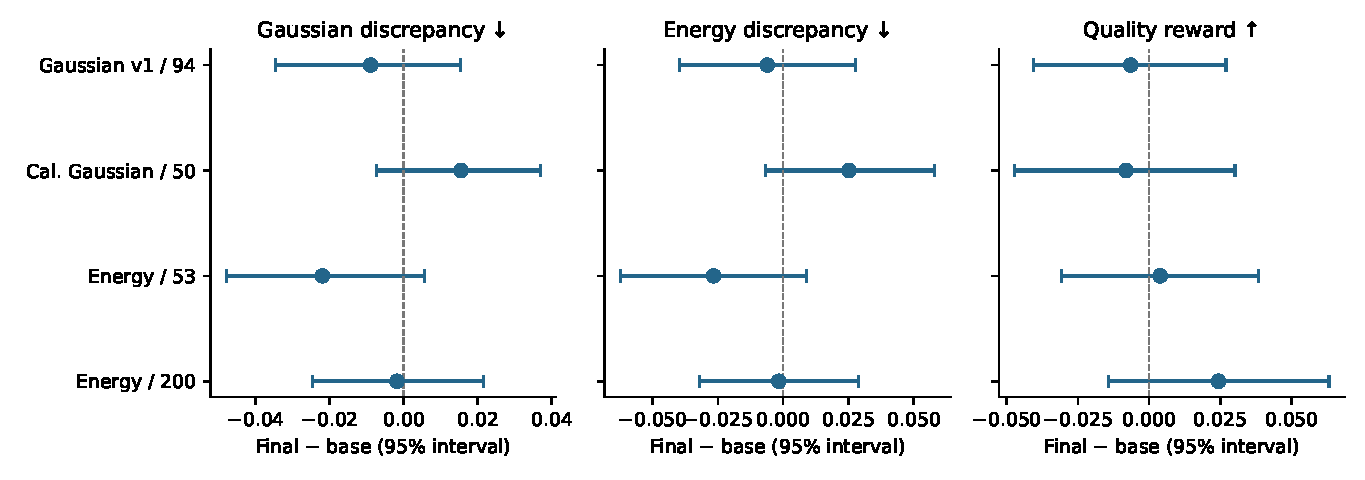
\includegraphics[width=\linewidth]{figures/semantic-changes.pdf}
 \caption{Paired question-level changes from the shared instruction baseline.
 Whiskers are exploratory bootstrap intervals (Table~\ref{tab:semantic-ci-new});
 every interval crosses zero. The 53- and 200-update energy points belong
 to one training trajectory.}
 \label{fig:semanticchanges}
\end{figure}
\begin{figure}[htbp]
 \centering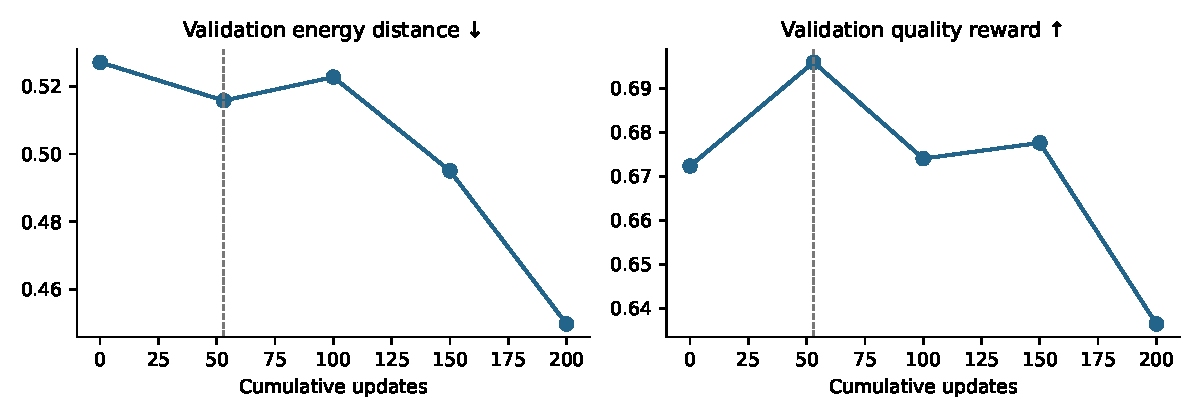
\includegraphics[width=\linewidth]{figures/energy-validation.pdf}
 \caption{Energy-run validation probes: ten questions, four answers each.
 The dashed line marks the update-53 checkpoint resumed by the continuation.
 These validation values use different questions from the final test and
 must not be compared as the same curve. Lines join saved probes only;
 they do not imply monotonic training progress.}
 \label{fig:energyvalidation}
\end{figure}
\FloatBarrier

\subsection{Four-question distribution-only fitting diagnostic}
To isolate limited in-sample fitting, a fresh base actor is trained on
four fixed eligible training questions, with 16 independent answers per
question per update (64 globally). Eligibility requires a single-turn
5--100-word prompt, both references 80--350 words, and reference-length
ratio at most two. Sorted eligible IDs are selected with seed 42;
four unseen original-validation questions are selected with seed 43.
The original 19-question test set is unused in this diagnostic.

Quality credit is exactly zero, with no reward scorer or quality judge
loaded. The retained objective is
\begin{equation}
 \mathcal L_{\mathrm{diag}}=
 \frac{0.5s_E\,\E_c D_E(P_c^{\mathrm{ref}},Q_{\theta,c})
      +0.002\,\E_c\KL(\pi_\theta\Vert\pi_0)}{1.502}.
 \label{eq:diagnosticloss}
\end{equation}
The divisor is deliberately unchanged when quality is removed. Centered
policy KL, fixed features/references and energy scale are retained.
The new schedule uses five warmup updates and a planned 100-step cosine
decay, cut off by a 70-minute policy-stage limit. The job completes
17 updates and 1,088 answers in a scheduler time of 1h18m37s.
This is a fresh small-question fitting test, not an ablation that changes
only the quality coefficient of the prior 102-question run.

Seen evaluation uses 32 answers per question (128 total), unseen 16
(64 total), with matched RNG isolated from training.
Seen energy distance falls 0.52614 to 0.50614 (3.80\%), with three of
four questions improving; intermediate update 10 is 0.5197.
The four-question mean-change interval is $[-0.0546,0.0111]$.
Unseen distance rises 0.58786 to 0.59691 (1.54\%), with mean-change
interval $[-0.0086,0.0277]$ (Table~\ref{tab:diagnostic-new}).
The evidence supports a modest, uncertain fitting signal and no
demonstrated generalization. It neither proves that fitting is
impossible nor establishes that the quality reward caused earlier
matching difficulty. Quality was not measured here.
\begin{table}[htbp]
\centering\small
\caption{Distribution-only diagnostic: four fixed training questions (seen), 32 evaluation answers each; four validation questions (unseen), 16 each. Quality is neither rewarded nor measured.}\label{tab:diagnostic-new}
\begin{tabular}{@{}lrrrr@{}}
\toprule
Scope / policy & Gaussian & Energy & Words & EOS (\%)\\
\midrule
Seen base & 0.4447 & 0.5261 & 561.6 & 81.2\\
Seen RL & 0.4282 & 0.5061 & 561.6 & 79.7\\
Unseen base & 0.4478 & 0.5879 & 469.3 & 57.8\\
Unseen RL & 0.4543 & 0.5969 & 458.8 & 59.4\\
\bottomrule
\end{tabular}
\end{table}


\subsection{Post hoc word and character distribution audits}
The following CPU analyses reuse saved diagnostic generations without
new sampling. Each compares outputs with the same exact question's
two references and averages question metrics equally. Word targets
pool references by word counts, unlike equal-answer weighting of the
semantic prototypes. All words enter numerical metrics; display-only
stopword filtering does not alter them. Forward KL uses total generated
pseudocount mass one. JSD and total variation are unsmoothed, with
an OTHER category for out-of-reference items.

\begin{table}[htbp]
\centering\small
\caption{Post hoc exact-question word matching on saved diagnostic outputs. Both reference answers are pooled by word count; question metrics are averaged equally. KL uses total generated pseudocount mass one; JSD and TV are unsmoothed with OTHER.}\label{tab:word-audit-new}
\begin{tabular}{@{}lrrr@{}}
\toprule
Scope / policy & Word KL & Word JSD & Word TV\\
\midrule
Seen base & 1.3325 & 0.2726 & 0.5478\\
Seen RL & 1.2785 & 0.2712 & 0.5483\\
Unseen base & 1.6379 & 0.3003 & 0.5923\\
Unseen RL & 1.6590 & 0.3005 & 0.5931\\
\bottomrule
\end{tabular}
\end{table}


Seen word KL falls by 4.05\%, but JSD changes only slightly and TV
worsens slightly. Unseen word KL, JSD and TV all worsen
(Table~\ref{tab:word-audit-new}). Matching an embedding objective does
not ensure matching lexical marginals, even with question-specific
references. These are post hoc JSD measurements, not a JSD training arm.

The character audit uses two explicit feature choices: raw
case-sensitive Unicode code points including whitespace, punctuation
and code; and lowercase English letters a--z only. References are
pooled by character count. With the same smoothing/OTHER conventions,
raw seen KL slightly worsens, while letters-only KL slightly improves
on both scopes (Table~\ref{tab:character-audit-new}). Raw unseen KL
increases from 0.18580 to 0.18955; its recorded four-question bootstrap
interval for the change is $[0.00076,0.00754]$. The other three
character-KL intervals include zero. These exploratory, post hoc
four-question summaries do not include training-seed or reference
uncertainty and are not corrected for multiple comparisons. Agreement
on common letters is particularly weak evidence for correct code,
vocabulary matching or semantic coverage.
\begin{table}[htbp]
\centering\scriptsize
\caption{CPU-only character-unigram audit of the same diagnostic samples. Each pair of columns is base $\to$ RL. Raw counts preserve case, spaces, newlines and punctuation; letters retain lowercase a--z only. Reference pooling is by character count; KL smoothing and OTHER follow the word audit.}\label{tab:character-audit-new}
\begin{tabular}{@{}lrrrrrrr@{}}
\toprule
Scope & Features & KL base & KL RL & JS base & JS RL & TV base & TV RL\\
\midrule
Seen & Raw Unicode & 0.09141 & 0.09165 & 0.02760 & 0.02781 & 0.11746 & 0.11695\\
Seen & Letters a--z & 0.01922 & 0.01877 & 0.00475 & 0.00463 & 0.07160 & 0.06916\\
Unseen & Raw Unicode & 0.18580 & 0.18955 & 0.03999 & 0.04111 & 0.16946 & 0.17085\\
Unseen & Letters a--z & 0.02560 & 0.02476 & 0.00635 & 0.00614 & 0.08031 & 0.07821\\
\bottomrule
\end{tabular}
\end{table}


\subsection{Recorded evidence and interpretation}
The text sequence contains both promising and negative results. The
Shakespeare trials improve distribution diagnostics and their shared
training judge; later HelpSteer trials do not establish a robust joint
benefit under stronger, separate model audits. Conditional reference
matching removes the conceptual mismatch of comparing unrelated questions,
but two references, frozen features and small conditional batches remain
restrictive. Calibration changes coefficient balance; centering preserves
the expected KL gradient. Neither implementation correctness nor a
reasonable objective guarantees a measurable policy improvement in the
available budget.

The source package includes the exact comparison/audit JSONs, configs,
source hashes, question-level semantic statistics, bootstrap settings,
and generated vector figures. The character audit is a local CPU record
with hashes verified against the committed diagnostic samples. All
training runs logged to the \texttt{stochastic-llm} W\&B project under
\texttt{yash2007-university-of-washington}; the included run records link
to the historical jobs. The source snapshot is repository commit
\texttt{deb5c8e} plus the recorded local character audit and manuscript
analysis. These records support reproducibility; upstream model/data
overlap, one seed, repeated diagnostic inspection and absence of new
human ratings remain material limits.

\FloatBarrier
\section{Discussion and limitations}
\paragraph{The result is a pilot, not a controlled comparison of algorithms.}
RL receives additional compute after SFT. We have not run an equal-compute
SFT continuation, a format-only control, a direct soft-KL full-model
experiment, multiple training seeds, or an ablation of reference
regularization and leave-one-out credit assignment. The experiment cannot
establish that RL is uniquely responsible for the gains or is more
efficient than supervised alternatives. Test prompts are not used for
optimization or checkpoint choice, but repeated future use of this test
set would weaken its value as an untouched benchmark.

\paragraph{The reward sees coarse marginal structure.}
Bin matching does not determine within-bin density, exact numerical precision,
or the magnitude of values inside open-ended tail bins. Finite batches and
pseudocount smoothing introduce bias and variance. Good histogram reward
can therefore coexist with errors in KS, Wasserstein, tails, and support.
We do not claim an exact KL between continuous laws. Generalization to
unseen numerical families is mixed. The numerical results alone do not
establish natural-language transfer; the completed text studies use
different targets and instruction-model initializations.
The MMD variant compares answer-feature distributions within the exact
question. Its two-reference target and frozen representation impose
different limitations. The completed semantic trials do not establish
reliable simultaneous gains in distribution matching and answer quality.
CPU sensitivity checks alone do not establish semantic correctness or
diversity in generated text.

\paragraph{The model remains substantially worse than a numerical sampler.}
A SciPy reference, rounded identically and matched to SFT valid counts,
has median KS 0.024720 and normalized Wasserstein 0.011348 over 20
repetitions per prompt. The RL medians are approximately 5.1 and 8.9
times these values. This reference is a finite-sample scale comparison,
not an exact lower bound or an RL-specific sample-count-matched control.
For explicit mathematical distributions, ordinary numerical samplers
remain the appropriate operational baseline.

\paragraph{Randomness, independence, and retention are separate claims.}
Training reshapes how a policy uses decoder pseudorandomness; it does
not create a new entropy source. A deterministic decoding procedure
cannot sample a nondegenerate target merely because weights were
fine-tuned. Fresh contexts remove conversational feedback between
requests but do not constitute a comprehensive statistical test of
independence, serial correlation, or cryptographic unpredictability.
We also do not measure general language ability or reasoning retention.

\section{Conclusion}
In one Qwen2.5-3B experiment, sampled-target SFT establishes a usable
numeric-output baseline, and a subsequent batch-KL-reward REINFORCE stage
adds a small average improvement in held-out distribution fidelity.
The average test KL reduction is 2.24\%, with larger median reductions
and heterogeneous transfer. The most useful next experiments are
replicated seeds, equal-compute supervised controls, and explicit tests
of tail accuracy, dependence, and capability retention. The current
evidence supports further investigation of distribution-level rewards,
without establishing a reliable general-purpose internal sampler.
The completed text sequence shows that improvements depend on the target
and measurement protocol. Shakespeare trials improve their training judge
and lexical matching, but the HelpSteer word-target and semantic trials do
not establish robust joint quality/distribution gains. Conditional MMD
addresses prompt relevance while matching only two equal-weight reference
prototypes. The early energy-matching improvement largely disappears with
longer training; removing quality yields only a modest fitting signal on
four seen questions, without demonstrated generalization. Replicated,
matched-budget comparisons against quality-only RL and SFT on the same
references, plus task correctness and human evaluation, are needed.

\begin{samepage}
\section*{Reproducibility and research assistance}
The public repository contains source, configs, recorded per-prompt metrics,
all 200,000 SFT/RL test generations, text-policy evaluation samples, and
W\&B links. The numerical-study snapshot is commit \texttt{27fad3e};
completed text records are included through \texttt{deb5c8e}, with the
local character-frequency audit separately hashed. Configs, compact
dataset manifests, audit reports, comparison JSONs and implementation
hashes are included in the source archive. Tables and vector figures
are generated from recorded files; the new semantic question-bootstrap
analysis is reproducible with its saved seed and per-question CSV.
Appendix~\ref{app:records} provides numerical version and artifact
details. Code development, analysis, and manuscript drafting were assisted
by an AI coding assistant. No additional full-model experiment was run
to prepare this manuscript.
\end{samepage}

\clearpage
\begingroup
\small
\setlength{\bibsep}{3pt}
\bibliographystyle{plainnat}
\bibliography{references}
\endgroup
\clearpage
\appendix
\section{Distribution definitions and dataset construction}
\label{app:distributions}
All target laws use the following parameter conventions. Densities are zero
outside the stated support; discrete formulas are probability masses.
\begin{align}
 \text{Normal: }\quad
 p(x)&=\frac{1}{\sigma\sqrt{2\pi}}
       \exp\!\left[-\frac{(x-\mu)^2}{2\sigma^2}\right],
       &&x\in\R,\\
 \text{Uniform: }\quad p(x)&=\frac{1}{b-a},&&a\leq x\leq b,\\
 \text{Exponential: }\quad p(x)&=\lambda e^{-\lambda x},&&x\geq0,\\
 \text{Beta: }\quad p(x)&=\frac{x^{a-1}(1-x)^{b-1}}{\mathrm B(a,b)},
       &&0<x<1,\\
 \text{Gamma: }\quad p(x)&=\frac{x^{k-1}e^{-x/s}}{\Gamma(k)s^k},&&x>0,\\
 \text{Binomial: }\quad p(x)&=\binom{n}{x}\rho^x(1-\rho)^{n-x},
       &&x\in\{0,\ldots,n\},\\
 \text{Weibull: }\quad p(x)&=\frac{k}{s}\left(\frac{x}{s}\right)^{k-1}
                e^{-(x/s)^k},&&x>0,\\
 \text{Poisson: }\quad p(x)&=e^{-\lambda}\frac{\lambda^x}{x!},
       &&x\in\{0,1,\ldots\}.
\end{align}
Here $\mathrm B(a,b)=\Gamma(a)\Gamma(b)/\Gamma(a+b)$. Gamma and Weibull
use shape/scale conventions, while exponential and Poisson use rates.
Support endpoints with zero continuous probability do not affect sampling.

Parameters are drawn independently and uniformly from the ranges in
Table~\ref{tab:ranges}, then rounded to five decimals. For binomial $n$,
the integer ranges are inclusive. Training and validation use the same
range rules but disjoint exact parameter combinations. The held-out
family ranges are used only for their test prompts.

\begin{table}[htbp]
\centering\small
\caption{Parameter-generation ranges. $U[a,b]$ denotes a continuous uniform
draw before parameter rounding. The uniform family's width is $w=b-a$.}
\label{tab:ranges}
\begin{tabular}{@{}lp{0.37\linewidth}p{0.37\linewidth}@{}}
\toprule
Family & Training / validation / new wording & Unseen parameters or families\\
\midrule
Normal & $\mu\sim U[-5,5]$, $\sigma\sim U[0.3,3]$ &
 $\mu\sim U[6,9]$, $\sigma\sim U[3.5,5]$\\
Uniform & $a\sim U[-5,2]$, $w\sim U[0.5,8]$ &
 $a\sim U[4,7]$, $w\sim U[9,12]$\\
Exponential & $\lambda\sim U[0.2,3]$ & $\lambda\sim U[3.5,5]$\\
Beta & $a,b\sim U[0.5,5]$ & $a,b\sim U[6,9]$\\
Gamma & $k\sim U[0.5,5]$, $s\sim U[0.3,3]$ &
 $k\sim U[6,9]$, $s\sim U[3.5,5]$\\
Binomial & $n\in\{5,\ldots,50\}$, $\rho\sim U[0.1,0.9]$ &
 $n\in\{55,\ldots,80\}$, $\rho\sim U[0.1,0.9]$\\
Weibull & Not used & $k\sim U[0.6,3]$, $s\sim U[0.5,4]$\\
Poisson & Not used & $\lambda\sim U[0.5,20]$\\
\bottomrule
\end{tabular}
\end{table}

The dataset seed is 20261117. The three prompt templates are:
\par\noindent\begin{minipage}{\linewidth}
\begin{quote}\small
\textbf{Training template 0:} Sample exactly one number from [distribution
description]. Output only the number.\newline Answer:\par
\textbf{Training template 1:} Generate one random draw from [distribution
description]. Return only its numeric value.\newline Answer:\par
\textbf{Held-out template 2:} I need a single independent observation drawn
according to [distribution description].\newline Number:
\end{quote}
\end{minipage}\par
Each label is followed by a newline. Descriptions spell out the parameter
names, for example ``a normal distribution with mean 7.83271 and standard
deviation 3.98876.'' Exact prompts, rather than this illustrative parameter
example, are stored in the committed test-case file. Training-family
selection cycles through six families; test-category selection cycles
through the three conditions while avoiding a coupling that would omit
families. Validation contains 160 configurations (1,280 target answers for
SFT); the RL probes use its first 12 configurations, two from each family.

\section{Gradient and objective details}
\subsection{Quantile bins and invalid responses}
\label{app:bins}
With a numeric-bin budget $K_{\max}=32$, begin with internal quantiles
$F_c^{-1}(j/32)$, $j=1,\ldots,31$. For a continuous law, round each to
the output grid and place the bin boundary a half-grid above it:
\begin{equation}
 e_j=\operatorname{round}_{\delta}\!\left(F_c^{-1}(j/32)\right)+\delta/2.
\end{equation}
Remove duplicate boundaries, CDF values at 0 or 1, and boundaries giving
zero mass. Numeric-bin masses are successive differences of
$[0,F_c(e_1),\ldots,F_c(e_{K-1}),1]$. These boundaries separate rounded
grid outputs, so CDF differences account for the rounded target mass.

For a discrete law with a finite support of at most 32 integers, all
adjacent support values are separated by half-integer boundaries. For
larger or infinite discrete supports, unique quantiles plus $1/2$ define
boundaries, followed by the same CDF-difference construction. Bin
assignment uses right-sided boundary search. A finite parsed number is
invalid for the reward if it is outside support (with half-grid tolerance
for continuous laws), or noninteger for a discrete law. Malformed text
and unfinished completions are also invalid.

The penalty for invalid mass can be seen at the population histogram
level. If $q_\bot<1$ and $\overline q_j=q_j/(1-q_\bot)$ normalizes the
numeric bins, then
\begin{equation}
 \KL(P\Vert Q)=\KL(P\Vert\overline Q)-\log(1-q_\bot).
 \label{eq:invalidpenalty}
\end{equation}
Thus ignoring the zero-target-mass term does not mean ignoring invalid
outputs; the loss still penalizes the probability diverted away from
valid bins. In implementation, the same normalization effect operates on
the smoothed empirical histogram.

\subsection{Unbiasedness of the leave-one-out policy gradient}
Fix a prompt $c$ and let the joint sampling law be
$\prod_i\pi_\theta(Y_i\mid c)$. Differentiating the expected batch reward
gives
\begin{align}
 \nabla_\theta\E R_N
 &=\sum_{Y_{1:N}} R_N\,
   \nabla_\theta\prod_i\pi_\theta(Y_i\mid c)\\
 &=\E\!\left[R_N\sum_i\nabla_\theta\log\pi_\theta(Y_i\mid c)\right].
\end{align}
For $b_i=R_{N-1}(c,Y_{-i})$, independence conditional on the prompt implies
\begin{align}
 \E[b_i\nabla_\theta\log\pi_\theta(Y_i\mid c)]
 &=\E_{Y_{-i}}\!\left[b_i\,
       \E_{Y_i}\nabla_\theta\log\pi_\theta(Y_i\mid c)\right]\\
 &=\E_{Y_{-i}}[b_i\nabla_\theta 1]=0.
\end{align}
Although the baseline's distribution changes with $\theta$, it is used as
a stop-gradient control variate; no baseline derivative is included.
This establishes Equation~\eqref{eq:groupgradient}. It relies on fresh
on-policy samples, consistent actor likelihoods, and the stated
conditional independence assumption. Reusing the same samples for multiple
unadjusted actor steps would break this on-policy justification.

\subsection{Closed-form leave-one-out advantage}
Write $j_i$ for the bin of action $i$, $n_{j_i}\geq1$ for its group count,
and $B$ for all categories, including invalid. Expanding the reward as
\begin{equation}
 R_N=-\sum_{j:p_j>0}p_j\log p_j
       +\sum_{j:p_j>0}p_j\log(n_j+\alpha)-\log(N+\alpha B)
\end{equation}
shows that removing one action only changes its selected count and the
normalizer. Therefore
\begin{equation}
 R_N-R_{N-1}=
 \log\frac{N-1+\alpha B}{N+\alpha B}
 +p_{j_i}\log\frac{n_{j_i}+\alpha}{n_{j_i}-1+\alpha}.
 \label{eq:closedadvantage}
\end{equation}
The implementation computes all advantages by this expression rather
than recomputing $N$ full histograms. If the action is invalid,
$p_{j_i}=0$ and its advantage is negative. Multiplying by $N$ and
averaging sequence losses recovers the group sum in
Equation~\eqref{eq:groupgradient}. Unit tests compare this estimator
against exact outcome enumeration on a small categorical group.

\subsection{What finite-sample histogram optimization does and does not imply}
\label{app:finite}
Let $q_j$ be the true model probability of histogram category $j$ at a
fixed prompt. Each marginal count $M_j$ has a binomial distribution
$\operatorname{Binomial}(N,q_j)$, even though the complete count vector is
multinomial. The expected reward is exactly
\begin{equation}
 \E R_N=-\sum_{j:p_j>0}p_j\log p_j-\log(N+\alpha B)
       +\sum_{j:p_j>0}p_j\E_{M_j}\log(M_j+\alpha).
 \label{eq:expectedreward}
\end{equation}
The expectation of a log count differs from the log of its expectation.
Consequently, maximizing the finite-$N$ reward is not identical to
minimizing $\KL(P\Vert Q)$, and its optimum need not be exactly $Q=P$.
The estimator's unbiased policy gradient is for this finite-sample
objective. As $N$ grows with fixed $B$ and $\alpha$, the empirical
smoothed histogram converges to $Q$; if all positive-target bins have
positive model probability, the realized KL converges to population bin
KL. This remains a statement about bins, not within-bin densities.

For a continuous target, an unsmoothed empirical measure places mass on a
finite set whereas the target has density over an interval. Directly
treating that empirical measure as a continuous density makes the
forward KL ill-defined or infinite. Explicit binning supplies the common
finite measurable partition needed by our implemented reward. A kernel
density alternative would introduce bandwidth and tail assumptions; we
do not use one here.

\subsection{Reference-KL score-function derivative}
\label{app:reference}
For fixed reference policy $\pi_0$ on the same capped completion space,
\begin{align}
 K(\theta)&=\sum_y\pi_\theta(y\mid c)
                  \log\frac{\pi_\theta(y\mid c)}{\pi_0(y\mid c)},\\
 \nabla_\theta K
 &=\E_{y\sim\pi_\theta}
   \left[\left(\log\frac{\pi_\theta(y\mid c)}{\pi_0(y\mid c)}+1\right)
            \nabla_\theta\log\pi_\theta(y\mid c)\right]\\
 &=\E_{y\sim\pi_\theta}
   \left[\log\frac{\pi_\theta(y\mid c)}{\pi_0(y\mid c)}
            \nabla_\theta\log\pi_\theta(y\mid c)\right].
\end{align}
The last step uses zero expected policy score. This is why
Equation~\eqref{eq:surrogate} subtracts the detached log-ratio from the
reward coefficient. Simply backpropagating an on-policy sampled log
ratio while treating sampled paths as fixed would omit the distribution's
score contribution. Both adapters share frozen base weights, while the
reference LoRA weights stay frozen. Disabling dropout for generation and
likelihood recomputation is necessary to score the sampled policy
consistently in this implementation.

\subsection{Direct soft-target KL: implemented, not a completed experiment}
For completeness, the code also supports supervision from a finite
canonical target law $P^{\mathrm{fin}}$ with at most 1,001 output strings.
For continuous laws, a rounded grid spans underlying quantiles 0.001 to
0.999; CDF differences define masses and edge bins absorb outer tails.
Discrete support is represented or coarsened under the same point budget.
Each output's token sequence, including EOS, is inserted into a prefix
trie. If $s$ is a target prefix, define
\begin{equation}
 P^{\mathrm{fin}}(v\mid s,c)=
 \frac{\sum_{y:sv\preceq y}P^{\mathrm{fin}}(y\mid c)}
      {\sum_{y:s\preceq y}P^{\mathrm{fin}}(y\mid c)}.
\end{equation}
Along target-sampled paths, the expected sum of next-token forward KLs
satisfies the chain rule
\begin{equation}
 \E_{Y\sim P^{\mathrm{fin}}}\sum_{t=1}^{T(Y)}
 \KL\!\left(P^{\mathrm{fin}}(\cdot\mid Y_{<t},c)
          \Vert\pi_\theta(\cdot\mid Y_{<t},c)\right)
 =\KL(P^{\mathrm{fin}}\Vert\pi_\theta).
\end{equation}
The model's softmax normalizer includes the full vocabulary; it is not
renormalized to valid trie children. Invalid output mass is therefore
penalized. The code sums losses over prefixes and averages over sampled
paths. The default uses three paths per training configuration, giving
6,000 paths, with a 64-trie cache. This is teacher-supervised distribution
matching, not a reward from model-generated samples. Its finite target
also differs from the full rounded law used by SFT and evaluation. No
full-model soft-KL results are included in this paper.

\section{Extended numerical results}
\label{app:extended}
\begin{table}[htbp]
\centering\small
\caption{Paired prompt-bootstrap differences, RL minus SFT. Negative
differences favor RL. Intervals use 10,000 resamples of the 100 prompt
indices and percentile endpoints. They do not incorporate training-seed
variability or multiple-comparison correction.}
\begin{tabular}{@{}llrr@{}}
\toprule
Metric & Aggregate & Difference & Exploratory 95\% interval\\
\midrule
Histogram KL & Mean & -0.005107 & [-0.008401, -0.001804] \\
Histogram KL & Median & -0.013447 & [-0.021973, +0.000740] \\
KS distance & Mean & -0.005296 & [-0.008375, -0.002172] \\
KS distance & Median & -0.012387 & [-0.022164, -0.000011] \\
Normalized Wasserstein & Mean & -0.003660 & [-0.006756, -0.000684] \\
Normalized Wasserstein & Median & -0.010959 & [-0.016946, +0.002674] \\
\bottomrule

\end{tabular}
\end{table}

\begin{table}[htbp]
\centering\small\setlength{\tabcolsep}{5pt}
\caption{Response quality over 100,000 requests per checkpoint.
Violations are valid numeric answers outside support or noninteger for
a discrete target. Truncation is measured over all requests.}
\label{tab:quality}
\begin{tabular}{@{}lrrrrr@{}}
\toprule
Policy & Valid count & Validity & Violations & Violations / valid & Truncated\\
\midrule
Pretrained & 6,838 & 6.838\% & 1,359 & 19.874\% & 88.625\% \\
SFT & 98,677 & 98.677\% & 1,330 & 1.348\% & 0.648\% \\
SFT + RL & 98,591 & 98.591\% & 1,208 & 1.225\% & 0.674\% \\
\bottomrule

\end{tabular}
\end{table}

\begin{table}[htbp]
\centering\small
\caption{All recorded RL validation probes: 12 fixed configurations,
256 draws each. The final tested adapter is update 250. The best mean KL
occurs at update 225, whose adapter was retained but not test-evaluated.}
\label{tab:validation}
\begin{tabular}{@{}rrrrr@{}}
\toprule
Update & Mean histogram KL & Median KS & Median normalized $W_1$ & Validity\\
\midrule
0 & 0.070539 & 0.068078 & 0.039160 & 100.00\% \\
25 & 0.066361 & 0.070032 & 0.034210 & 100.00\% \\
50 & 0.072817 & 0.069250 & 0.039073 & 100.00\% \\
75 & 0.072290 & 0.061455 & 0.034566 & 100.00\% \\
100 & 0.069355 & 0.064310 & 0.028803 & 100.00\% \\
125 & 0.067104 & 0.060269 & 0.028083 & 100.00\% \\
150 & 0.066409 & 0.063268 & 0.033190 & 100.00\% \\
175 & 0.065829 & 0.063264 & 0.031405 & 100.00\% \\
200 & 0.067312 & 0.065217 & 0.029034 & 100.00\% \\
225 & 0.064350 & 0.070032 & 0.031264 & 100.00\% \\
250 & 0.065246 & 0.056670 & 0.030995 & 100.00\% \\
\bottomrule

\end{tabular}
\end{table}

All 100 prompt-level base/SFT/RL outcomes are included in the source
package's supplementary CSV. The paper uses the already-recorded test
metrics and the post-hoc histogram KL analysis; it does not select a
different checkpoint or decoding configuration to improve the results.
The repository additionally records canonical formatting, repeated-value
rates, sample means and standard deviations, support violations, and
metric overflow flags per prompt. These diagnostics are descriptive,
not a comprehensive test of random-number quality.

\FloatBarrier
\section{Artifacts and reproduction}
\label{app:records}
The numeric code and records are available at
\href{https://github.com/YashSolanki2007/llm-random-number-generator/tree/27fad3ec875afb2941f34ab873e8394ae24f25e8}{repository commit \texttt{27fad3e}}.
It includes all 200,000 SFT/RL test responses, per-prompt metrics,
training history, configs, and provenance hashes. The earlier SFT records
include base metrics and two cases' raw responses. Training rollouts and
adapters remain in W\&B artifacts and cluster storage. This manuscript's
source archive includes generated tables, vector figures, the bibliography,
and a supplementary per-prompt CSV.

The production environment records PyTorch 2.8.0+cu126, Transformers
4.57.1, PEFT 0.17.1, Accelerate 1.10.1, NumPy 2.2.6, SciPy 1.15.3,
and W\&B 0.31.0, with CUDA 12.6 on an NVIDIA H200. Production training
and evaluation require online W\&B logging. No credentials are present
in this manuscript or its source archive.

\paragraph{Run records.}
\begin{itemize}
\item SFT training:
\href{https://forge.coreweave.com/wandb/yash2007-university-of-washington/stochastic-llm/runs/xcj01bg1}{\texttt{xcj01bg1}}.
\item Base and SFT evaluation:
\href{https://forge.coreweave.com/wandb/yash2007-university-of-washington/stochastic-llm/runs/rfddft7y}{\texttt{rfddft7y}} and
\href{https://forge.coreweave.com/wandb/yash2007-university-of-washington/stochastic-llm/runs/ao4xvmp5}{\texttt{ao4xvmp5}}.
\item RL training and evaluation:
\href{https://forge.coreweave.com/wandb/yash2007-university-of-washington/stochastic-llm/runs/tx91cho0}{\texttt{tx91cho0}} and
\href{https://forge.coreweave.com/wandb/yash2007-university-of-washington/stochastic-llm/runs/n9d9aegn}{\texttt{n9d9aegn}}.
\item Final SFT/RL comparison:
\href{https://forge.coreweave.com/wandb/yash2007-university-of-washington/stochastic-llm/runs/lyb3xv9l}{\texttt{lyb3xv9l}}.
\end{itemize}
The RL timing benchmark, training, and evaluation were Slurm jobs
493753, 493754, and 493755, respectively; all completed successfully.
These identifiers are provenance, not instructions to reuse outputs.

\paragraph{Regenerate analysis from the repository.}
The following commands require no GPU and create no online training run:
\begin{quote}\small\ttfamily
python -m pip install -e '.[dev,analysis]'\\
python -m pytest -q\\
python scripts/analyze\_rl\_results.py --recorded\\
python paper/generate\_assets.py
\end{quote}
The manuscript compiles independently of the experiment data. Regenerating
its tables and figures requires the repository records.

\end{document}
